\chapter{Metodologia}
\label{cap:metodologia}

Este capítulo descreve os procedimentos e decisões de projeto adotados no desenvolvimento do sistema integrado de bancada para ensaios de conjuntos motopropulsores. A metodologia está organizada em quatro frentes de trabalho interdependentes: \textit{Computer-Aided Design} (CAD), o Sistema Integrado da Bancada Aerodinâmica (SIBA) , a Interface de Usuário ( ou PC) e o Sistema de Aquisição do Motor Elétrico (SAME).  Para fins de resultados mais pertinentes à equipe Albatroz Aerodesign, designou-se o motor Scorpion A-5025-310Kv e a Bateria Lipo 6S de 3300mAh 40C, mostra na \autoref{fig:motor_batata}.

\begin{figure}[H]
    \centering
    \caption{Bateria e Motor}
    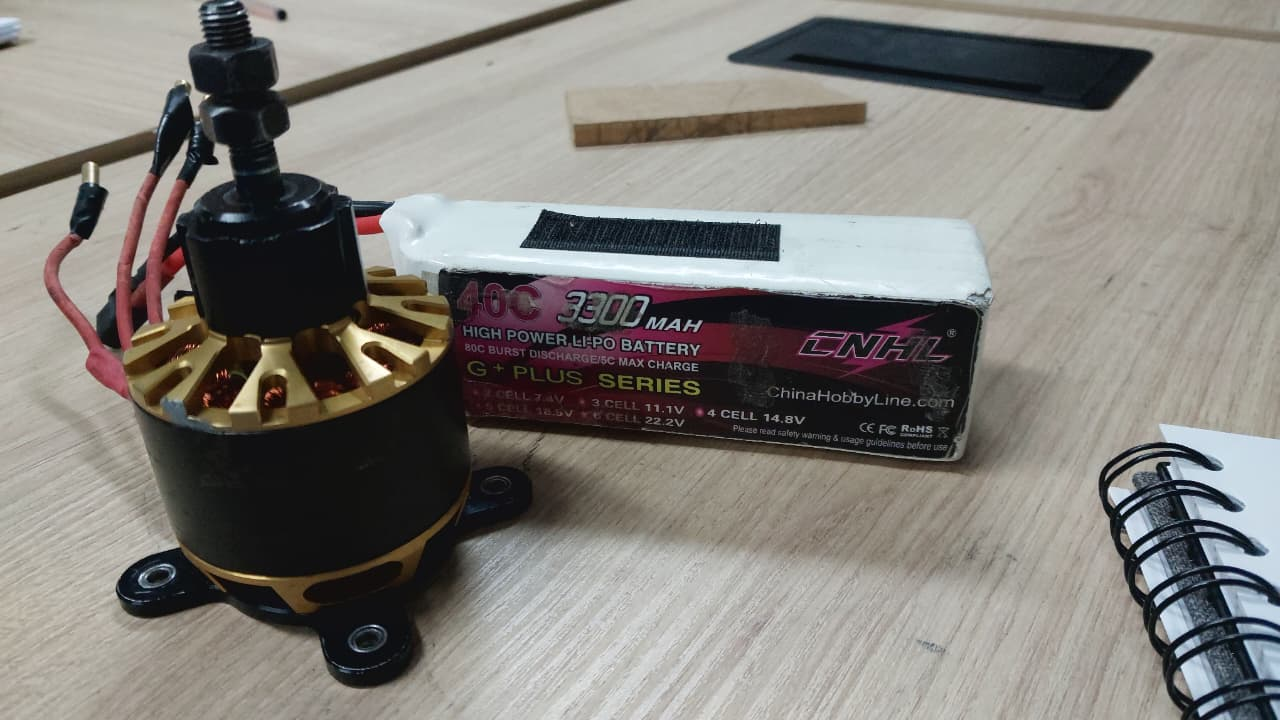
\includegraphics[width=0.5\linewidth]{Textuais/Imgs/Metodologia/Motor_batata.jpeg}
    \label{fig:motor_batata}

    Fonte: Autor (2026)
\end{figure}

A execução metodológica e a sequência lógica deste trabalho orientam-se pelo fluxo detalhado na \autoref{fig:TCC_planejmamento}. É imperativo notar a presença dos estágios Q1, Q2 e Q3: estes atuam como as principais janelas de transição do projeto, concentrando as deliberações e decisões mais críticas que fundamentam o desenvolvimento da pesquisa.

A etapa Q1 é a etapa de decisão de projeto, onde são definidas as restrições e definições de projeto, Q2 é a etapa de validação de cada uma das \textit{features} de forma individual, já Q3 é a finalização do projeto, marcando seu término.

\begin{figure}[H]
    \centering
    \caption{Metodologia Principal do TCC}
    
    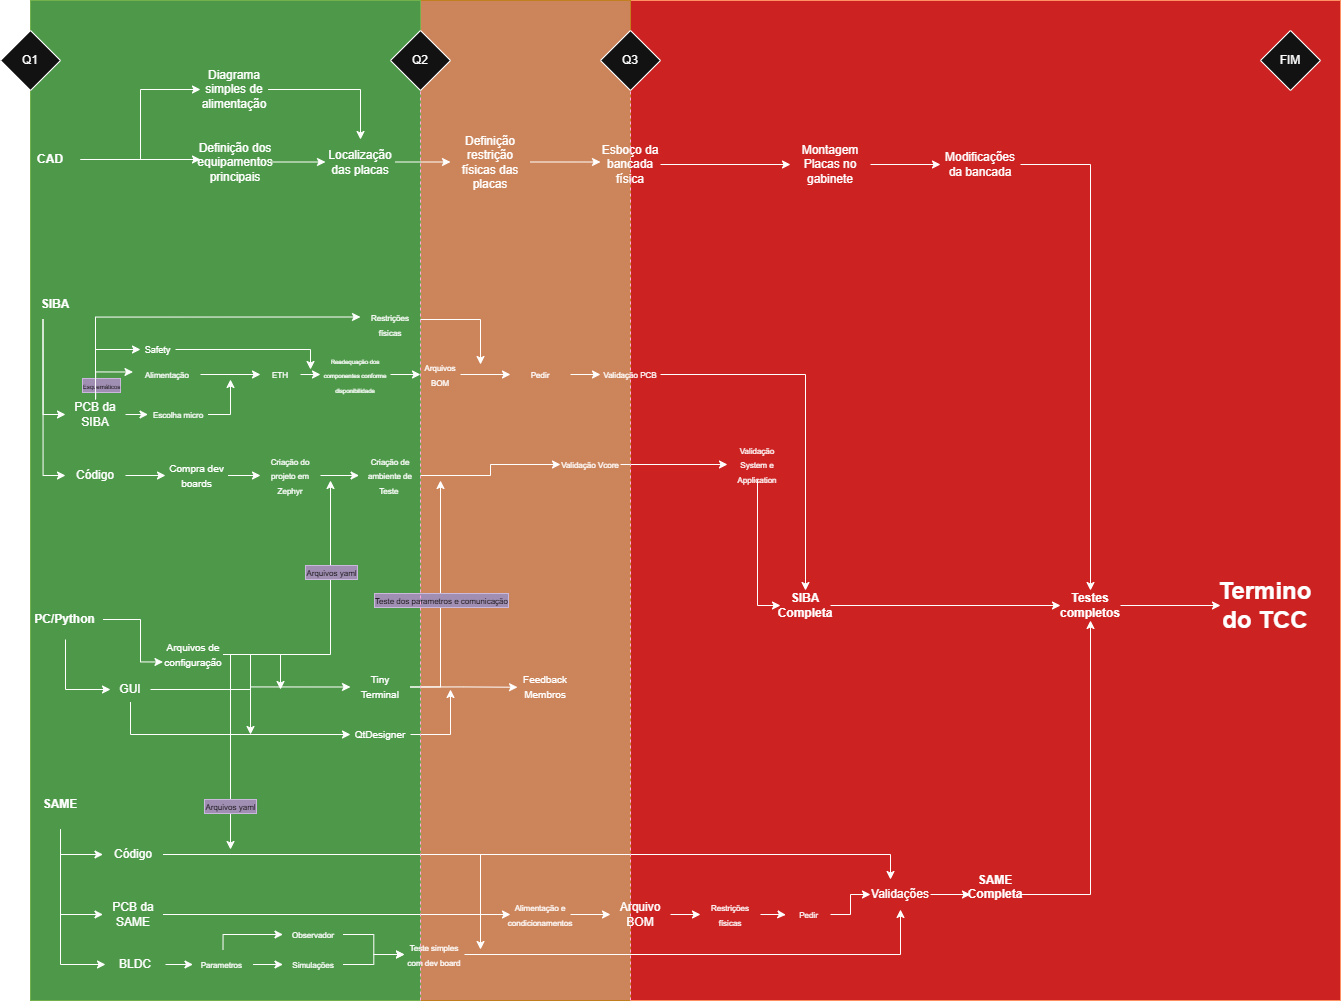
\includegraphics[angle=90, scale=0.45]{Textuais/Imgs/Metodologia/TCC Planejamento.png}
    \label{fig:TCC_planejmamento}

    Fonte: Autor (2026)
\end{figure}


\section{Declaração de uso de ferramentas de Inteligência Artificial}

Durante a elaboração deste trabalho, o autor utilizou ferramentas de
Inteligência Artificial Generativa como instrumento auxiliar, nas finalidades
e condições descritas a seguir:

\begin{itemize}
    \item \textbf{Revisão textual e formatação:} ChatGPT (OpenAI), Claude
    (Anthropic), Gemini (Google) e DeepSeek foram utilizados para auxiliar na
    revisão gramatical, na clareza da redação, na formatação de tabelas e
    equações em \LaTeX{} e na organização de seções do texto.

    \item \textbf{Apoio ao desenvolvimento e verificação de cálculos:} as mesmas
    ferramentas foram empregadas para conferência de cálculos e deduções
    previamente desenvolvidos pelo autor, e como apoio à discussão de conceitos
    técnicos.

    \item \textbf{Desenvolvimento de software:} Claude Code (Anthropic), por meio
    de interface de linha de comando (CLI), foi utilizado como assistente no
    desenvolvimento e na depuração de código, incluindo a geração de scripts em
    Python para automação de testes de software.
\end{itemize}

Todo o conteúdo produzido com auxílio dessas ferramentas foi revisado, editado
e validado pelo autor, que assume total responsabilidade pela precisão,
originalidade e integridade do conteúdo deste trabalho, bem como pelo
funcionamento e correção do código desenvolvido.

% ------------------------------------------------------------------ %
\section{Motor BLDC}
\label{sec:motor_bldc}

Para fins de resultados pertinentes à equipe Albatroz Aerodesign,designou-se o motor \textit{Scorpion A-5025-310Kv} como unidade sob ensaio. A caracterização do motor exige a identificação experimental de seus parâmetros elétricos e mecânicos, os quais alimentam tanto o modelo dinâmico quanto o observador de estados.

\subsection{Parâmetros Elétricos}
\label{sec:params_eletricos}

Para a determinação da resistência e da indutância de fase, emprega-se o ensaio de rotor bloqueado, cujo circuito equivalente está ilustrado na Figura \ref{fig:circuito_estrela_bldc}. O travamento mecânico do eixo impede a indução de forças contraeletromotrizes decorrentes de micro-oscilações, reduzindo o modelo elétrico do motor a uma malha puramente passiva em ligação estrela\footnote{Este equacionamento é válido independentemente do fechamento interno real da máquina. Para um motor fechado em delta, a impedância medida linha a linha equivale a duas fases em série em paralelo com a terceira ($Z_{linha} = \frac{2}{3}Z_{\Delta}$). Como a transformação para o modelo equivalente em estrela requer $Z_Y = \frac{Z_{\Delta}}{3}$, chega-se à mesma relação final $Z_Y = \frac{Z_{linha}}{2}$, permitindo modelar o motor a partir dos terminais como uma caixa preta.}.

\begin{figure}[H]
    \centering
    \caption{Circuito Equivalente do Motor BLDC (Rotor Bloqueado) }
    
    \begin{tikzpicture}[transform shape, american]
        % Ponto Neutro
        \node[circ] (N) at (0,0) {};
        \node[above left, xshift=-0.1cm] at (N) {$N$};

        % Fase U (Para Cima)
        \draw (N) to[american resistor, l=$R_{fase}$] (0,2) 
                  to[cute inductor, l=$L_{fase}$] (0,4) 
                  node[ocirc] (U) {} 
                  node[above] {Fase $U$};

        % Fase V (Para a Direita/Baixo) - Ângulo de -30°
        \draw (N) to[american resistor, l=$R_{fase}$] (1.732,-1) 
                  to[cute inductor, l=$L_{fase}$] (3.464,-2) 
                  node[ocirc] (V) {} 
                  node[right] {Fase $V$};

        % Fase W (Para a Esquerda/Baixo) - Ângulo de 210°
        \draw (N) to[american resistor, l_=$R_{fase}$] (-1.732,-1) 
                  to[cute inductor, l_=$L_{fase}$] (-3.464,-2) 
                  node[ocirc] (W) {} 
                  node[left] {Fase $W$};

        % --- Indicação do Ensaio (Medição Linha a Linha) ---
        
        % Linhas de chamada (tracejadas) saindo de U e V para a direita
        \draw[dashed, blue!70!black] (U) -- (5.5, 4);
        \draw[dashed, blue!70!black] (V) -- (5.5, -2);
        
        % Seta dupla indicando a medição com texto explicativo
        \draw[<->, blue!70!black, thick] (5.5, 3.9) -- node[fill=white, align=center, text=black] {Ensaio Linha a Linha \\ $V_{DC}, I_{DC}$ (Resistência) \\ $L_{linha}$ (Indutância) \\ \small \textit{Equivalente a 2 em série}} (5.5, -1.9);

        % Marcação do caminho da corrente para ficar mais didático (Opcional)
        \draw[->, red, thick, rounded corners=5mm] (0.5, 3.5) -- (0.5, 0.5) -- (3.0, -1.0) node[pos=0.8, above right] {$I_{ensaio}$};

    \end{tikzpicture}
    \label{fig:circuito_estrela_bldc}
    
    \small Fonte: Autor (2026)
\end{figure}

A resistência de fase é medida aplicando-se uma corrente contínua entre dois terminais do motor. Nesta condição, a reatância indutiva é nula e a queda de tensão ocorre integralmente sobre as resistências. Medindo-se a tensão ($V_{DC}$) e a corrente ($I_{DC}$), a resistência de fase equivalente é calculada por:

\begin{equation}
    R_{fase} = \frac{V_{DC}}{2\,I_{DC}}
    \label{eq:resistencia_fase}
\end{equation}


De maneira análoga, com o rotor ainda imobilizado, conduz-se o ensaio para a
obtenção da indutância de fase através do método da ressonância. Motores BLDC
aplicados em aeromodelismo, como o \textit{Scorpion A-5025}, geralmente possuem
ímãs montados na superfície do rotor (SPM --- \textit{Surface Permanent
Magnet}). O entreferro efetivamente uniforme característico dessa topologia
torna a saliência magnética insignificante, permitindo assumir que as
indutâncias de eixo direto ($L_d$) e em quadratura ($L_q$) são aproximadamente
iguais ($L_d \approx L_q \approx L_s$), onde $L_s$ é a indutância síncrona da
máquina \cite{Krishnan2017}.

Na ausência de um medidor LCR, o ensaio consiste em associar um capacitor de
valor conhecido ($C$) em paralelo com o enrolamento da máquina, formando um
circuito ressonante $LC$ alimentado por uma fonte senoidal de frequência
variável através de um resistor série $R$, conforme a
Figura~\ref{fig:circuito_ressonancia_v2}. Ao varrer a frequência da fonte até
atingir a frequência de ressonância ($f_r$), na qual a impedância do tanque
$LC$ é máxima e a tensão sobre ele atinge seu valor de pico, a indutância pode
ser estimada \cite{Fitzgerald2014}. A condição de ressonância corresponde ao
ponto em que a reatância do circuito se anula, restando apenas as componentes
resistivas. Após determinar a indutância equivalente medida entre dois
terminais ($L_{linha}$), a indutância de fase individual é obtida pela relação
de ressonância:

\begin{figure}[htbp]
    \centering
    \caption{Circuito de ensaio de ressonância: resistor $R$ em série com o
    paralelo $L$--$C$, com a tensão de ressonância medida sobre o tanque.}
    \label{fig:circuito_ressonancia_v2}
    \begin{circuitikz}[american, scale=1.1, transform shape]
        % ---- Fonte e resistor série (ramo superior) ----
        \draw (0,0) to[sV, l=$v_{in}$] (0,3);
        \draw (0,3) to[R, l=$R$, i>^=$i_{in}$] (3,3);
        % ---- Nó de medição (saída do gerador / topo do tanque) ----
        \node[circ] (A) at (3,3) {};
        \node[anchor=south] at (3,3.2) {\footnotesize nó A};
        % ---- Ramo do indutor ----
        \draw (A) to[L, l=$L_{fase}$] (3,0);
        % ---- Ramo do capacitor (em paralelo) ----
        \draw (A) -- (5.5,3);
        \draw (5.5,3) to[C, l=$C$] (5.5,0);
        % ---- Trilho de terra (retorno) ----
        \draw (0,0) -- (5.5,0);
        \node[circ] (G) at (3,0) {};
        \node[ground] at (1.5,0) {};
    \end{circuitikz}

    \fonte{Autor (2026).}
\end{figure}

\begin{equation}
    f_r = \frac{1}{2\pi\sqrt{L_{linha} \cdot C}}
    \implies
    L_{linha} = \frac{1}{C\,(2\pi f_r)^2}
    \label{eq:ressonancia_L}
\end{equation}

Considerando a topologia de conexão dos enrolamentos, a indutância de fase
individual é dada por:

\begin{equation}
    L_{fase} = \frac{L_{linha}}{2}
    \label{eq:indutancia_fase}
\end{equation}

Este valor de $L_{fase}$ é diretamente empregado como o parâmetro $L_s$ nas
equações de espaço de estados no referencial estacionário $\alpha\beta$.

\subsection{Parâmetros Mecânicos}
\label{sec:params_mecanicos}

A dinâmica mecânica do motor é governada pela equação de balanço de torques no eixo rotativo, como visto na \autoref{eq:bldc_mecanica}.

Para a caracterização experimental, o motor BLDC é acionado utilizando um Controlador Eletrônico de Velocidade (ESC) comercial. Como o torque eletromagnético ($T_e$) em motores de ímã permanente é proporcional à corrente de eixo em quadratura ($I_q$), a bancada de testes irá ser instrumentada para adquirir as correntes instantâneas de fase do motor. O esquema de \textit{hardware} e as formas de onda esperadas estão ilustrados na Figura \ref{fig:circuito_esc_correntes}.

\begin{figure}[H]
    \centering
    \caption{Esquema de Medição com ESC e Transformação de Correntes ($abc \to dq$)}
    
    % --- PARTE 1: CIRCUITO DE \textit{hardware} COM AJUSTES DE LEGENDA ---
    \begin{tikzpicture}[auto, node distance=2cm, >=latex']
        
        % --- Blocos principais ---
        \node [draw, rectangle, minimum height=3em, minimum width=4em] (bat) {Bateria};
        
        % Aumentei para 8em para comportar o deslocamento das fases com folga
        \node [draw, rectangle, minimum height=8em, minimum width=4em, right=of bat, node distance=2.5cm] (esc) {ESC};
        
        % BLDC posicionado à direita
        \node [draw, rectangle, rounded corners=8pt, minimum height=8em, minimum width=5em, right=of esc, node distance=6.5cm] (motor) {BLDC};
        
        % SAME/DAQ centralizado abaixo
        \node [draw, rectangle, minimum height=4em, minimum width=10em, below=of esc, node distance=4.5cm, xshift=3.25cm] (daq) {SAME / DAQ};

        % --- Conexões Bateria -> ESC ---
        \draw [thick] ([yshift=0.3cm]bat.east) -- node[above] {$V_{DC}$} ([yshift=0.3cm]esc.west);
        \draw [thick] ([yshift=-0.3cm]bat.east) -- node[below] {GND} ([yshift=-0.3cm]esc.west);

        % --- Coordenadas das Fases (A, B, C) ---
        % Deslocadas para cima (+0.5cm) para não bater no centro (0) do Eixo
        \coordinate (esc_a) at ([yshift=1.5cm]esc.east);
        \coordinate (esc_b) at ([yshift=0.5cm]esc.east);
        \coordinate (esc_c) at ([yshift=-0.5cm]esc.east);
        
        \coordinate (mot_a) at ([yshift=1.5cm]motor.west);
        \coordinate (mot_b) at ([yshift=0.5cm]motor.west);
        \coordinate (mot_c) at ([yshift=-0.5cm]motor.west);

        % --- Conexões das Fases ---
        \draw [thick] (esc_a) -- node[above, pos=0.5, font=\large\bfseries] {A} (mot_a);
        \draw [thick] (esc_b) -- node[above, pos=0.5, font=\large\bfseries] {B} (mot_b);
        \draw [thick] (esc_c) -- node[below, pos=0.5, font=\large\bfseries] {C} (mot_c);

        % --- Sensores de Corrente (Intercalados) ---
        % Sensor A (Violeta) próximo ao ESC
        \node [draw, circle, minimum size=0.45cm, inner sep=0pt, thick, fill=white] (sensA) at ([xshift=1.2cm]esc_a) {};
        % Sensor B (Teal) próximo ao Motor
        \node [draw, circle, minimum size=0.45cm, inner sep=0pt, thick, fill=white] (sensB) at ([xshift=1.5cm]esc_b) {};
        
        % --- Sensor de Posição Óptico (No Eixo Central) ---
        \node [draw, rectangle, minimum height=2em, right=of motor, node distance=2.2cm] (enc) {Sensor};
        % O Eixo sai do centro exato (0), onde agora não há fios
        \draw [thick, dashed] (motor.east) -- node[above] {Eixo} (enc.west);

        % --- Conexões de Dados para o SAME (Intercaladas) ---
        % Sensor A desce mais (3.5cm)
        \draw [->, dashed, violet, thick] (sensA.south) -- ++(0,-3.5) -| ([xshift=-1.2cm]daq.north);
        
        % Sensor B desce menos (1.8cm)
        \draw [->, dashed, teal, thick] (sensB.south) -- ++(0,-3.5) -| ([xshift=-0.9cm]daq.north);
        
        % Sensor de posição vem pela lateral
        \draw [->, dashed, thick] (enc.south) |- (daq.east) node[pos=0.8, above] {$\theta, \omega$};
        
        % --- Label de transformação ---
        \node [below, font=\scriptsize, text width=5cm, align=center] at (daq.south) { $I_c = -(I_a + I_b)$ \\ Clarke \& Park $\to I_d, I_q$};

    \end{tikzpicture}
    \label{fig:circuito_esc_intercalado}
    
    \vspace{0.8cm} % Espaço entre o circuito e os gráficos

    % --- PARTE 2: GRÁFICOS DAS CORRENTES COM AJUSTES DE EIXO ---
    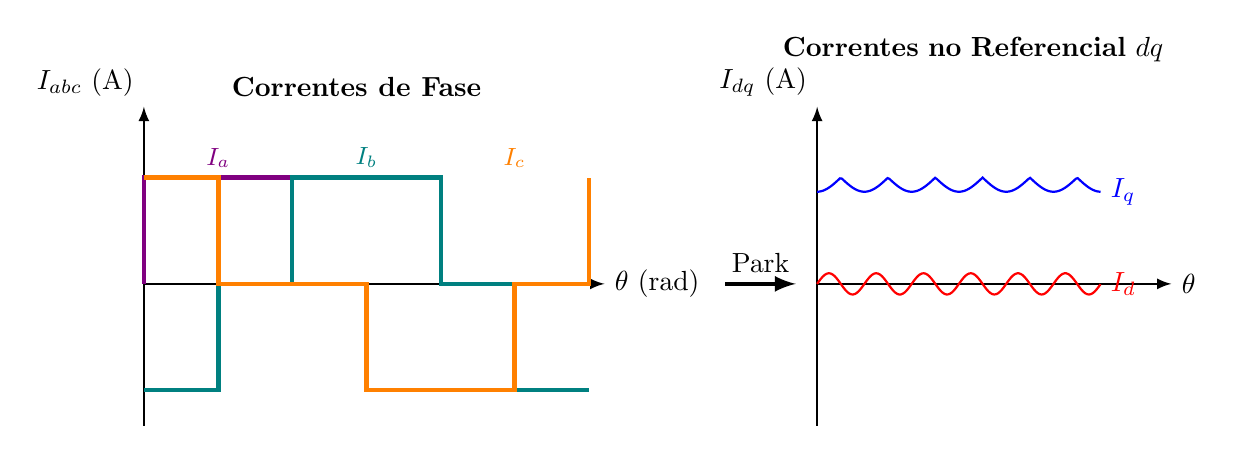
\begin{tikzpicture}[scale=0.9, >=latex]
        
        \begin{scope}[xshift=0cm]
            \draw[->, thick] (0,-2) -- (0,2.5) node[above left] {$I_{abc}$ (A)};
            \draw[->, thick] (0,0) -- (6.5,0) node[right] {$\theta$ (rad)};
            
            % Curva Ia (120 graus ligada, 60 desligada)
            \draw[ultra thick, violet] (0,0) -- (0,1.5) -- (2.09,1.5) -- (2.09,0) -- (3.14,0) -- (3.14,-1.5) -- (5.23,-1.5) -- (5.23,0) -- (6.28,0);
            \node[above, violet, font=\small\bfseries] at (1.05, 1.5) {$I_a$};

            % Curva Ib (Atrasada 120 graus)
            \draw[ultra thick, teal] (0,-1.5) -- (1.05,-1.5) -- (1.05,0) -- (2.09,0) -- (2.09,1.5) -- (4.19,1.5) -- (4.19,0) -- (5.23,0) -- (5.23,-1.5) -- (6.28,-1.5);
            \node[above, teal, font=\small\bfseries] at (3.14, 1.5) {$I_b$};

            % Curva Ic (Adiantada 120 graus)
            \draw[ultra thick, orange] (0,1.5) -- (1.05,1.5) -- (1.05,0) -- (3.14,0) -- (3.14,-1.5) -- (5.23,-1.5) -- (5.23,0) -- (6.28,0) -- (6.28,1.5);
            \node[above, orange, font=\small\bfseries] at (5.23, 1.5) {$I_c$};
            
            \node[above] at (3, 2.5) {\textbf{Correntes de Fase}};
        \end{scope}

        % --- Seta de Transformação ---
        \draw[->, ultra thick] (8.2, 0) -- node[above, black] {Park} (9.2, 0);

        % --- Gráfico 2: Correntes FOC (dq) com RIPPLE ---
        \begin{scope}[xshift=9.5cm]
            \draw[->, thick] (0,-2) -- (0,2.5) node[above left] {$I_{dq}$ (A)};
            \draw[->, thick] (0,0) -- (5,0) node[right] {$\theta$};
            
            % Curva Iq (Com ripple de comutação - 6 pulsos)
            \draw[thick, blue, domain=0:4, samples=150] plot (\x, {1.5 - 0.2*abs(cos(4.71*\x r))}) node[right] {$I_q$};
            
            % Curva Id (Oscilando em torno de zero)
            \draw[thick, red, domain=0:4, samples=150] plot (\x, {0.15*sin(9.42*\x r)}) node[right] {$I_d$};
            
            \node[above, text width=5cm, align=center] at (2.2, 3) {\textbf{Correntes no Referencial $dq$}};
        \end{scope}

    \end{tikzpicture}
    
    \label{fig:circuito_esc_correntes}
    \small Fonte: Autor (2026)
\end{figure}

Através do Sistema de Aquisição do Motor Elétrico (SAME), lê-se as correntes de pelo menos duas fases (ex: $I_a$ e $I_b$). Considerando que não há conexão de neutro, a terceira corrente é obtida por $I_c = -(I_a + I_b)$. Sincronizando essas leituras com a posição angular elétrica do rotor ($\theta_e$) --- obtida indiretamente pela medição do sensor óptico --- aplica-se as transformadas de Clarke e Park (\textit{offline} ou \textit{online}) para mapear as grandezas do referencial trifásico estacionário ($abc$) para o referencial síncrono girante ($dq$) \footnote{Devido à natureza da comutação trapezoidal (6-step) do ESC utilizado, as correntes de fase apresentam harmônicos que resultam em oscilações (\textit{ripple}) nas componentes $I_d$ e $I_q$ após a transformada de Park. Para os cálculos de caracterização, utiliza-se o valor médio filtrado de $I_q$, que representa a componente fundamental do torque eletromagnético médio em regime permanente.}. 

\subsubsection{Coeficiente de Atrito Viscoso}
\label{sec:atrito_viscoso}

Para extrair os coeficientes de atrito ($B$ e $\tau_c$) \footnote{O atrito de Coulomb ($\tau_c$) representa uma parcela de torque constante necessária para vencer a fricção estática e cinética dos rolamentos}, estabiliza-se a rotação do motor a vazio em múltiplos patamares. Em regime permanente ($\frac{d\omega_m}{dt} = 0$), o torque eletromagnético anula exatamente as perdas mecânicas:

\begin{equation}
    T_{e,k}= B\omega_{m,k} + \tau_c
    \label{eq:ensaio_vazio_iq}
\end{equation}

Os parâmetros $B$ e $\tau_c$ são obtidos através de uma regressão linear sobre os pontos experimentais médios $(\omega_{m,k}, T_{e,k})$ para cada patamar de rotação, o $\omega_{m,k}$ é medido através de um tacômetro digital para validação.

\subsubsection{Momento de Inércia}
\label{sec:momento_inercia}

Com o atrito estabelecido, o momento de inércia ($J$) é estimado pelo ensaio de desaceleração livre (\textit{coast-down}). Ao atingir a rotação nominal máxima, a aceleração via ESC é cortada. Sem excitação externa, as correntes caem a zero ($I_q = 0$), zerando o torque motriz. A dinâmica de parada é descrita por:

\begin{equation}
    J \frac{d\omega_m}{dt} = - B\omega_m - \tau_c
    \label{eq:coast_down_iq}
\end{equation}

O sensor óptico registra a curva de desaceleração $\omega_m(t)$. Isolando $J$ e calculando a derivada $\frac{d\omega_m}{dt}$ a partir dos dados adquiridos na região de decaimento, extrai-se o momento de inércia do conjunto rotativo.


\subsection{Parametrização do SMO}
\label{sec:param_smo}

Com os parâmetros intrínsecos do motor obtidos, resta o problema de selecionar os ganhos deslizantes ($K_{s1}$, $K_{s2}$) e o polo do estimador ($K_t$). Esses parâmetros condicionam características antagônicas: ganhos elevados aceleram a convergência do erro de predição de corrente, porém amplificam o conteúdo harmônico injetado na BEMF; o polo $K_t$ atenua esse ruído ao custo de atraso de fase dependente da frequência elétrica. Como a frequência elétrica varia ao longo do envelope de operação, não há um conjunto de ganhos trivialmente ótimo, e o ajuste manual revela-se laborioso e pouco reprodutível. Esses fatores motivaram a adoção de um procedimento de ajuste automático \textit{(autotuning)} offline, capaz de ser
reaplicado sistematicamente a diferentes conjuntos motopropulsores --- requisito
central para uma bancada de caracterização que se pretende geral.

O procedimento é conduzido sobre a planta computacional do conjunto
motopropulsor, que fornece as referências de torque e velocidade. Ao longo desta seção, essas grandezas geradas pela planta simulada são designadas ``reais'', em contraposição às estimativas produzidas pelo observador; não se trata, portanto, de medições experimentais, mas da referência sintética contra a qual o estimador é ajustado.

O objetivo físico do observador, neste contexto, é estimar com fidelidade as
grandezas de saída do conjunto: o torque de eixo e a velocidade angular. São
essas as variáveis posteriormente empregadas na identificação dos coeficientes
aerodinâmicos. Por essa razão, ao invés de penalizar grandezas internas do
estimador --- como o erro angular, que o PLL já torna pouco discriminante ---, a
função-custo foi formulada como o \textit{seguimento} direto do torque e da
velocidade \cite{hermuche2023funcoes, datacamp2025cost}, mantendo o procedimento
agnóstico aos detalhes internos do observador e, portanto, transferível a outros
motores.

A avaliação ocorre sobre os trechos em regime permanente de cada patamar de
velocidade. Para um patamar $q$, a \autoref{eq:termos_seguimento} define o erro
de seguimento de torque ($g_{T,q}$), a partir das amostras de torque real
($\Tau_{q,n}$) e estimado ($\hat{\Tau}_{q,n}$), e o erro relativo de velocidade
($g_{\omega,q}$), das velocidades médias real ($\varpi_q$) e estimada
($\hat{\varpi}_q$). O termo de torque emprega a função de perda de Huber
($\ell_\delta$), que combina sensibilidade quadrática próxima ao acerto com
robustez linear aos desvios grandes, atenuando o impacto das quedas periódicas
de observabilidade do SMO durante as comutações do inversor sem descartá-las por
completo:
%
\begin{equation}
    g_{T,q} = \frac{1}{N_q}\sum_{n=1}^{N_q}
        \ell_\delta\!\big( \hat{\Tau}_{q,n} - \Tau_{q,n} \big),
    \qquad
    g_{\omega,q} = \frac{\big|\, \hat{\varpi}_q - \varpi_q \,\big|}{|\varpi_q|},
    \label{eq:termos_seguimento}
\end{equation}
%
onde $N_q$ é o número de amostras do patamar e $\ell_\delta(r) = \tfrac{1}{2}r^2$
para $|r|\le\delta$ e $\ell_\delta(r) = \delta\,(|r|-\tfrac{1}{2}\delta)$ caso
contrário. A função-custo agregada, apresentada na
\autoref{eq:custo_autotuning}, é a média ponderada desses erros sobre os $M$
patamares avaliados:
%
\begin{equation}
    J(\mathbf{x}) = \frac{1}{M}\sum_{q=1}^{M}
        \Big( w_T\,g_{T,q} + w_\omega\,g_{\omega,q}\Big),
    \label{eq:custo_autotuning}
\end{equation}
%
com pesos $w_T = \num{1,0}$ e $w_\omega = \num{0,5}$, priorizando deliberadamente
a fidelidade do torque, grandeza de maior interesse para a caracterização
propulsiva. Cabe ressaltar que o valor numérico de $J$ não constitui uma medida
de exatidão global do estimador: a topologia é fortemente não linear e o erro
varia entre patamares, de modo que $J$ deve ser entendido apenas como o índice
relativo que orienta a busca, e não como um erro percentual absoluto.

Na discretização por Euler progressivo, os ganhos atuam sobre a dinâmica do
observador na forma dos produtos definidos na
\autoref{eq:discretizacao_coeff_smo}, de modo que um mesmo comportamento
dinâmico corresponde a valores de $K$ inversamente proporcionais a $T_s$.
Otimizar $K$ diretamente atrelaria o resultado ao passo específico da simulação,
comprometendo sua transferência ao \textit{firmware}, cujo período de execução é
ditado pelo hardware de aquisição. Por essa razão, a otimização é conduzida
sobre os ganhos discretizados $\Gamma$, invariantes ao passo, recuperando-se o
ganho efetivamente embarcado por $K = \Gamma / T_s$ com o $T_s$ real da malha de
controle.

Para condicionar a busca, os parâmetros são otimizados em espaço logarítmico com
sinais fixos, escrevendo $\Gamma=(+1,-1,+1)\odot 10^{\mathbf{x}}$, o que
normaliza as três ordens de grandeza distintas e impõe por construção as
restrições de sinal $\Gamma_{s1}>0$, $\Gamma_{s2}<0$ e $\Gamma_{t}>0$. A
minimização emprega o algoritmo de Evolução Diferencial
(\autoref{alg:autotuning}), executando a simulação em um horizonte reduzido que
cobre os patamares mais exigentes.

\begin{algorithm}[H]
\caption{Ajuste automático de ganhos (offline)}
\label{alg:autotuning}
\begin{algorithmic}[1]
\Require ponto inicial $\mathbf{x}_0$, limites $\mathcal{B}$, perfil reduzido
\Function{Custo}{$\mathbf{x}$}
    \State $\Gamma \gets (+1,-1,+1)\odot 10^{\mathbf{x}}$
    \State $(K_{s1},K_{s2},K_t) \gets \Gamma / T_s$
    \State $\textbf{out} \gets$ \Call{Simular}{$K_{s1},K_{s2},K_t$}
    \If{$\textbf{out}$ não é finito} \State \Return penalidade elevada \EndIf
    \State \Return $J(\textbf{out})$ \Comment{Eq.~\eqref{eq:custo_autotuning}}
\EndFunction
\State $\mathbf{x}^{\star} \gets \displaystyle\operatorname*{arg\,min}_{\mathbf{x}\in\mathcal{B}}\ \textsc{Custo}(\mathbf{x})$
    \Comment{Evolução Diferencial}
\State \Return $\Gamma^{\star} = (+1,-1,+1)\odot 10^{\mathbf{x}^{\star}}$
\end{algorithmic}
\end{algorithm}

A natureza não-convexa de $J$, decorrente do \textit{chattering} e das saturações
da planta, justifica a adoção de um método de otimização livre de gradiente. Os
ganhos resultantes e a verificação de invariância ao passo são reportados na
\autoref{sec:autotuning}.

\section{Interface de Usuário e de Comunicação}

A comunicação do sistema é realizada via rede Ethernet estruturada com o auxílio de um \textit{switch}, conforme ilustrado na \autoref{fig:arquitetura_hardware}. A padronização do método de transmissão baseia-se no uso de endereçamento IP estático para as placas de aquisição e controle, o que simplifica a identificação dos dispositivos na rede e a integração com a interface. O protocolo adotado para a troca de pacotes é o UDP (\textit{User Datagram Protocol}), escolhido por sua baixa latência e menor sobrecarga de cabeçalho, características fundamentais para o monitoramento de telemetria em tempo real.

\begin{figure}[htbp]
    \centering
    \caption{Diagrama de Arquitetura de Comunicação e \textit{hardware}.}
    \resizebox{0.9\textwidth}{!}{
    \begin{tikzpicture}[
        node distance=1.5cm and 2cm,
        font=\sffamily,
        % Estilos das caixas principais
        box/.style={draw=black, thick, rounded corners, align=center, fill=none},
        % Estilos das caixas internas do Computador
        innerbox/.style={draw=black, thick, rounded corners, align=center, minimum height=1.2cm, fill=none},
        % Estilo das setas duplas
        arrow/.style={<->, >=stealth, thick, draw=black}
    ]

        % ==========================================
        % LADO ESQUERDO: SIBA e SAME
        % ==========================================
        \node[box, text width=4cm, minimum height=2.8cm] (siba) {
            \textbf{SIBA}\\[0.3cm] 
            Monitoramento\\da Bancada e\\Bateria
        };
        
        \node[box, text width=4cm, minimum height=2.8cm, below=0.5cm of siba] (same) {
            \textbf{SAME}\\[0.3cm] 
            Monitoramento\\do motor
        };

        % ==========================================
        % CENTRO: SWITCH DE REDE
        % ==========================================
        % Pega o ponto central entre SIBA e SAME para alinhar o Switch
        \path (siba) -- (same) coordinate[midway] (midLeft);
        
        \node[box, right=3cm of midLeft, minimum height=6.1cm, minimum width=1.0cm] (switch) {
            \rotatebox{90}{\textbf{SWITCH DE REDE}}
        };

        % ==========================================
        % LADO DIREITO: COMPUTADOR PYTHON E NÓS INTERNOS
        % ==========================================
        % Título do PC
        \node[right=2.5cm of switch, yshift=2cm, align=center, font=\sffamily\Large\bfseries] (pctitle) {Computador};
        
        % Bloco Observador
        \node[innerbox, text width=5cm, below=0.8cm of pctitle] (obs) {Interface de Usuário};
        
        % Blocos Plot, CSV, Terminal (Centralizados pelo CSV)
        \node[innerbox, minimum width=1.5cm, below=0.8cm of obs] (csv) {CSV};
        \node[innerbox, minimum width=1.5cm, left=0.3cm of csv] (plot) {Plot};
        \node[innerbox, minimum width=1.5cm, right=0.3cm of csv] (Terminal) {Terminal};

        % Caixa externa que engloba tudo do Computador
        \node[draw=black, thick, rounded corners, inner sep=0.6cm, fit=(pctitle) (obs) (plot) (csv) (Terminal)] (pc) {};

        % ==========================================
        % CONEXÕES (SETAS)
        % ==========================================
        % Seta SIBA <-> Switch (alinhada com o meio da SIBA)
        \draw[arrow] (siba.east) -- (switch.west |- siba.east);
        
        % Seta SAME <-> Switch (alinhada com o meio da SAME)
        \draw[arrow] (same.east) -- (switch.west |- same.east);
        
        % Seta Switch <-> Computador (alinhada com o meio do Switch)
        \draw[arrow] (switch.east) -- (pc.west |- switch.east);

    \end{tikzpicture}
    }
    \label{fig:arquitetura_hardware}

    Fonte: Autor (2026)
\end{figure}

Para garantir a fluidez da aplicação e evitar o congelamento da interface durante a recepção de dados em alta frequência, a arquitetura do \textit{software} foi paralelizada. A aplicação divide as responsabilidades em múltiplas \textit{threads}, isolando módulos críticos como a escuta de rede, a renderização da interface gráfica (GUI), a plotagem dos gráficos e o processamento do terminal de comandos.

A \autoref{fig:gui_metodologia} apresenta o diagrama da arquitetura lógica do \textit{software}, demonstrando o fluxo de comunicação entre as partes. O gerenciador de rede opera em segundo plano (\textit{background workers}), monitorando os \textit{sockets} UDP de forma assíncrona. Ao receber um pacote, os dados são decodificados e estruturados, disparando eventos (\textit{callbacks}) que atualizam os \textit{buffers} visuais e os registros de \textit{log}.

\begin{figure}[H]
    \centering
    \caption{Diagrama da Interface de Usuário e Comunicação}
    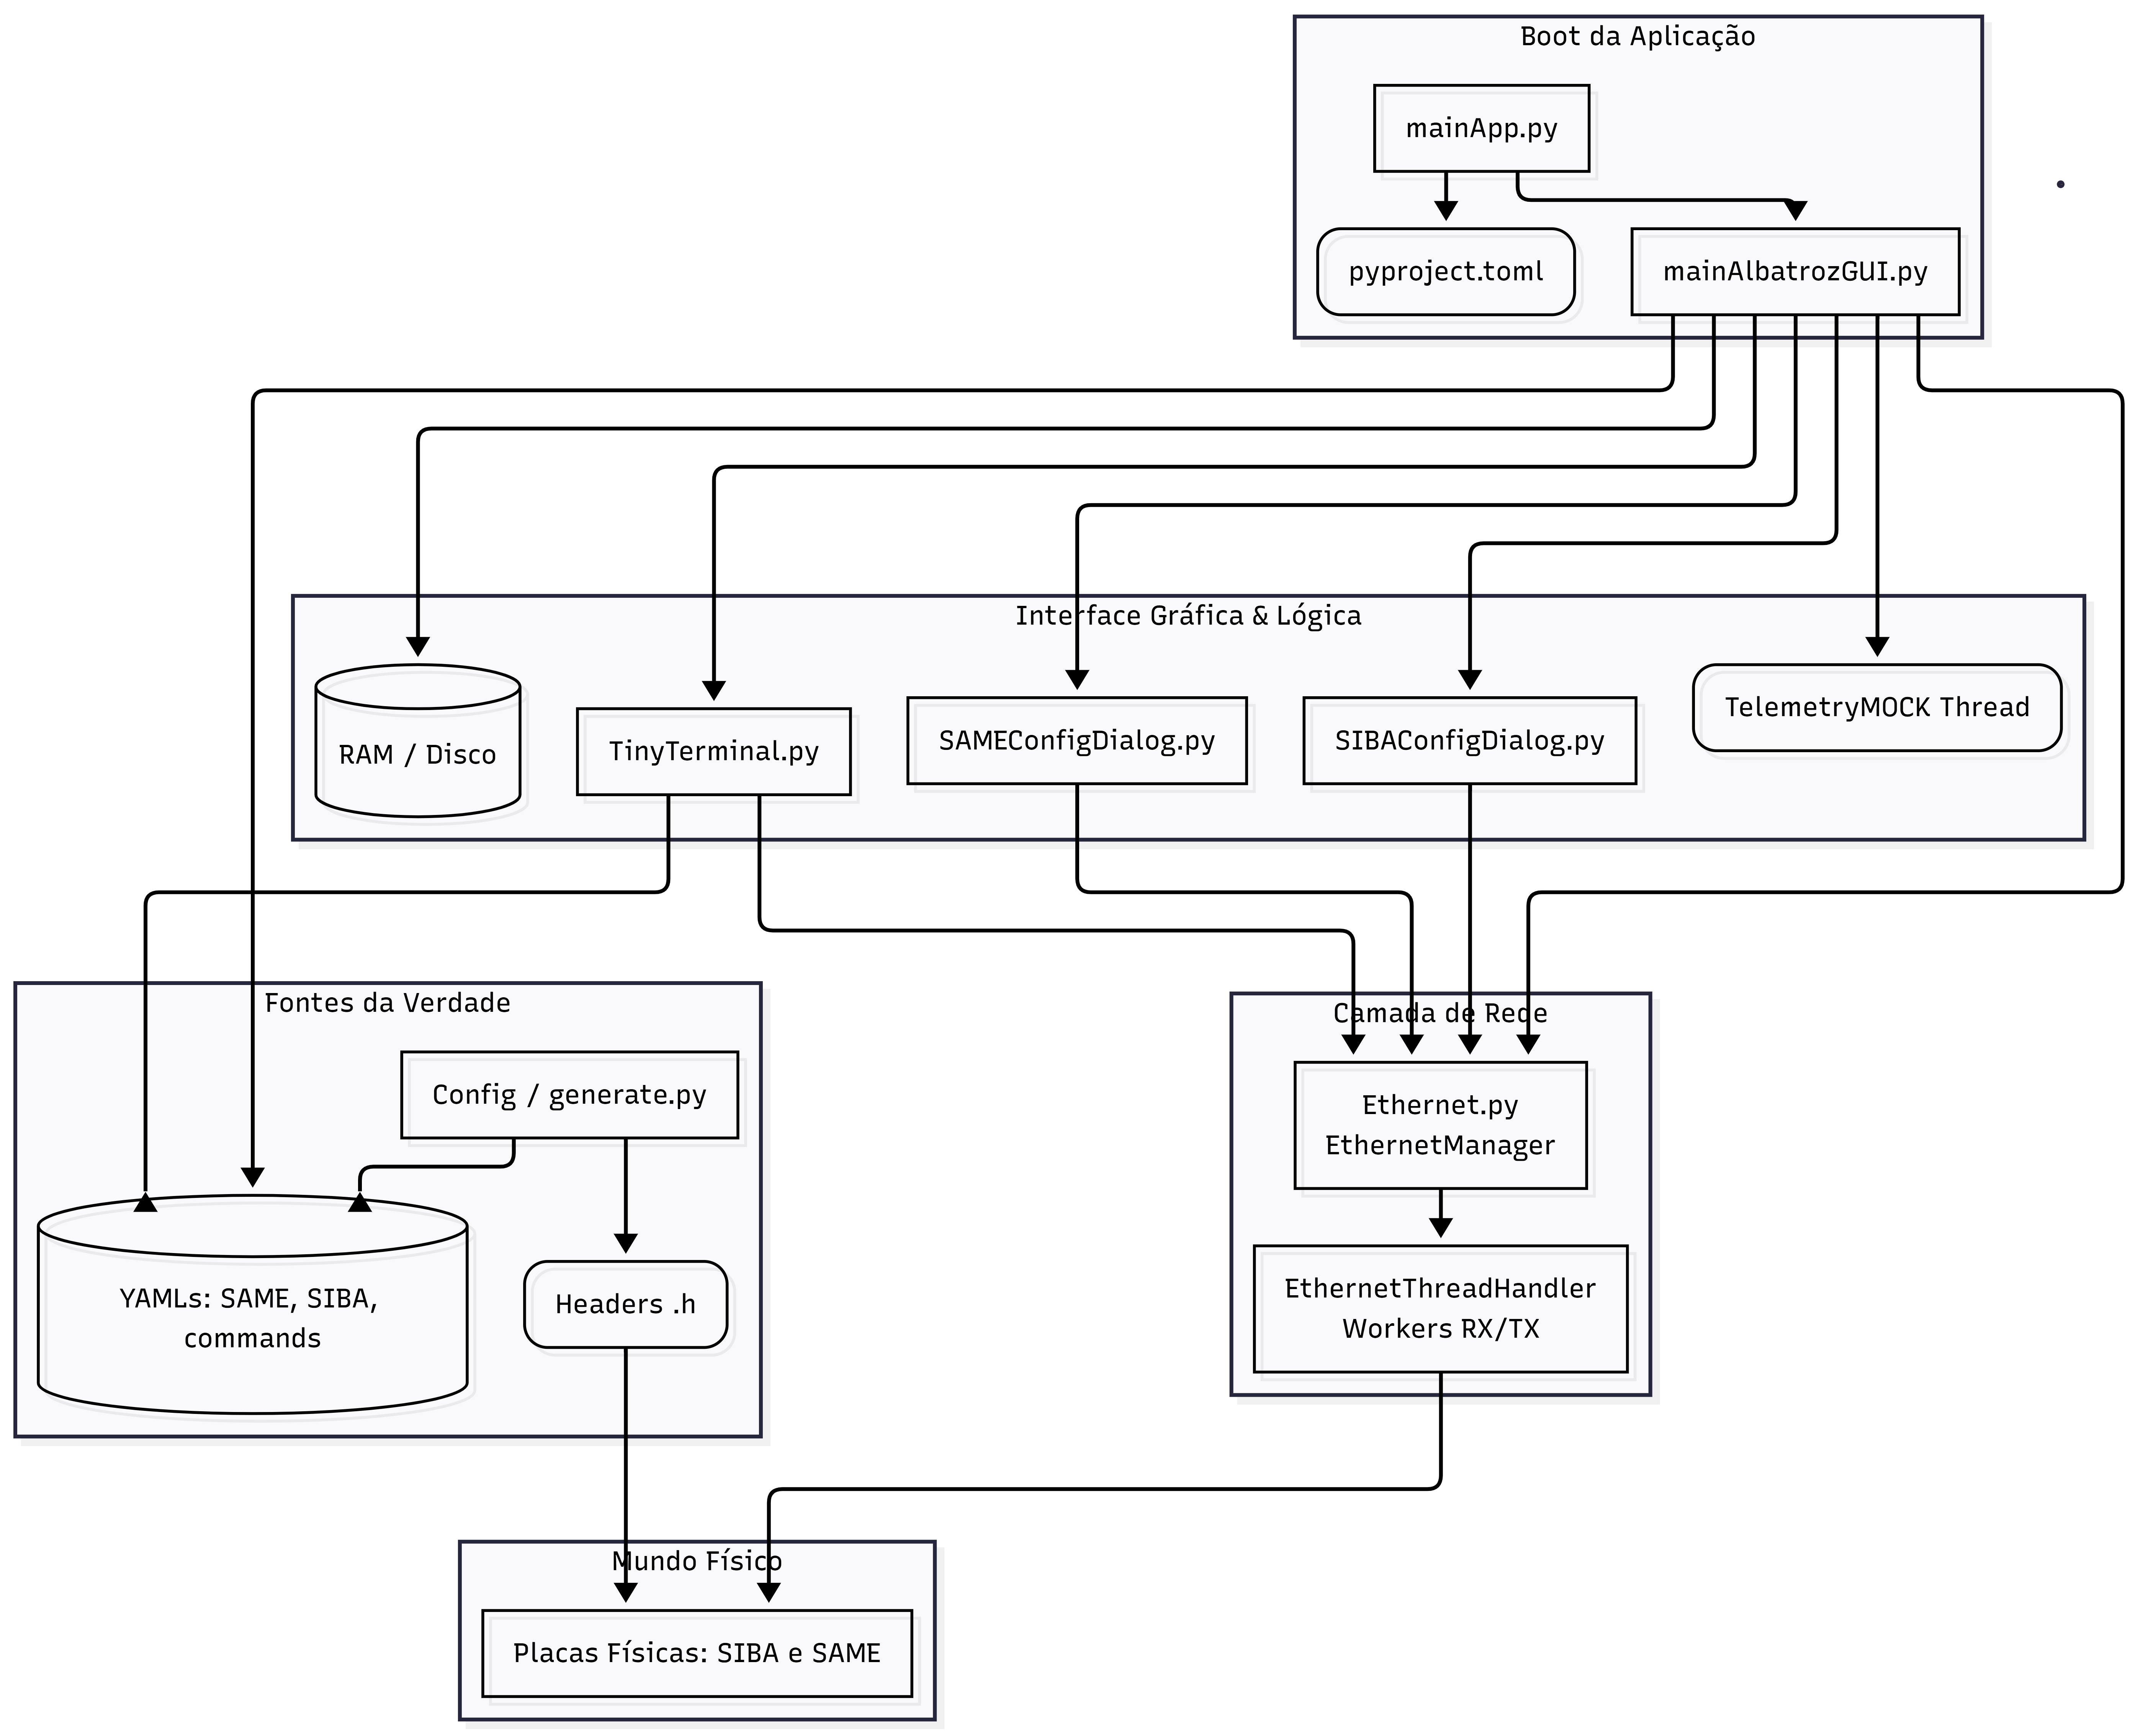
\includegraphics[width=0.7\linewidth]{Textuais/Imgs/Metodologia/GUI_diagrama.png}
    \label{fig:gui_metodologia}

    Fonte: Autor (2026)
\end{figure}

Para viabilizar a instrumentação e o controle da bancada, foi desenvolvida uma Interface de Operação e Supervisão utilizando o ecossistema \textit{PyQt}, integrando a ferramenta de \textit{design} gráfico \textit{Qt Designer} à linguagem \textit{Python}. A interface foi projetada para atuar como um centro de controle unificado, cumprindo os seguintes requisitos operacionais essenciais:

\begin{itemize}
    \item \textbf{Monitoramento em Tempo Real:} Visualização dinâmica de variáveis críticas para o diagnóstico imediato do comportamento dos motores e sensores;
    \item \textbf{Parametrização Interativa:} Capacidade de ajuste dinâmico dos parâmetros de controle das placas de processamento durante a operação, sem a necessidade de interrupção ou de novos \textit{uploads} de código;
    \item \textbf{Otimização do Desenvolvimento:} Fornecimento de um ambiente de abstração que simplifique a interação com os diversos nós (\textit{boards}) do sistema, acelerando os processos de teste e validação de \textit{hardware}.
\end{itemize}

Para que essa parametrização interativa e o monitoramento operem com alta confiabilidade, mitigando erros de interpretação de dados entre diferentes plataformas, o sistema adota uma estratégia de padronização baseada na linguagem de serialização YAML (\textit{YAML Ain't Markup Language}). A implementação utiliza arquivos de descrição que definem as estruturas fundamentais de telemetria (\textit{logs}), comandos (\textit{CMD}) e configurações da interface.

Como ilustrado na \autoref{fig:yaml_example_config}, essa abordagem estabelece os arquivos YAML (\textit{commands.yaml}, \textit{user\_prefs.yaml}, \textit{SAME.yaml} e \textit{SIBA.yaml}) como a fonte única da verdade do projeto. Enquanto a aplicação de alto nível em \textit{Python} consome esses arquivos para moldar a GUI e gerar os comandos padronizados, um \textit{script} auxiliar (\textit{generate.py}) processa as configurações exclusivas das placas (SAME e SIBA) para compilar automaticamente os arquivos de cabeçalho (\textit{headers} em C). Dessa forma, o \textit{firmware} dos microcontroladores e a aplicação \textit{desktop} compartilham a mesma lógica estrutural. Garante-se, assim, que qualquer alteração nos dados trafegados seja refletida instantaneamente em todas as instâncias do sistema, assegurando a integridade da comunicação.

\begin{figure}[H]
    \centering
    \caption{Fluxo de uso dos arquivos YAML para configuração integrada da GUI e do \textit{firmware}.}
    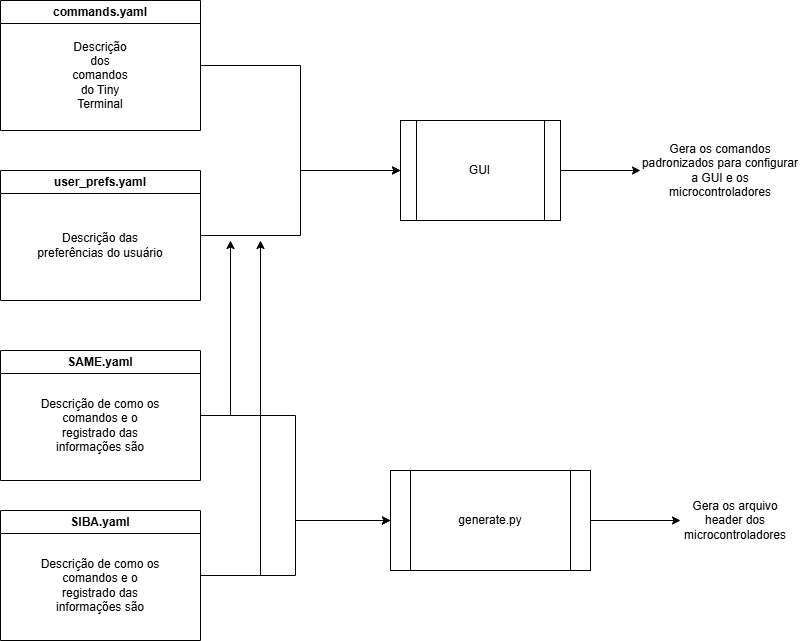
\includegraphics[width=0.8\linewidth]{Textuais/Imgs/Metodologia/YAML_uso.drawio.png}
    \label{fig:yaml_example_config}


    Fonte: Autor (2026).
\end{figure}


\section{Padronização das Placas}
Esta seção estabelece as diretrizes de projeto e as restrições metodológicas adotadas para o desenvolvimento das placas de aquisição e controle (SIBA e SAME). Visando otimizar os custos de manufatura e garantir a modularidade do sistema, por conta disso irá se usar placas de fenolite manufaturadas a mão, bem como módulos, placas de desenvolvimento e conversores comerciais.

Adotou-se o microcontrolador CH32V307VCT6 (WCH) como unidade de processamento
das placas SIBA e SAME. A escolha fundamenta-se em quatro critérios principais.
Primeiro, o conversor analógico-digital com taxa de até 1 Msps
atende à amostragem rápida de correntes e tensões exigida pela aquisição e pelo
controle. Segundo, a ampla memória disponível acomoda o \textit{firmware} sobre
o sistema operacional de tempo real Zephyr, as estruturas de dados de aquisição
e o processamento em ponto flutuante do controle vetorial e do observador, este
último amparado pela unidade de ponto flutuante (FPU) do núcleo RISC-V de
\SI{144}{\mega\hertz}. Terceiro, o dispositivo integra interface Ethernet
(MAC e PHY), detalhada adiante. Por fim, o baixo custo — cerca de
R\$30 por placa, ou aproximadamente R\$90 considerando
tributos de importação — viabiliza a produção de múltiplas unidades dentro das
restrições orçamentárias do projeto.

A interface Ethernet merece destaque por ter motivado a escolha. Durante o ano
de 2025, membros da equipe Albatroz Aerodesign identificaram a necessidade de um
método de comunicação mais simples e padronizado entre as placas de aquisição e
os computadores de ensaio. A conectividade por rede via cabo atende a essa
demanda: dispensa conversores de sinal intermediários, como adaptadores
UART-TTL (\textit{Universal Asynchronous Receiver/Transmitter} e \textit{Transistor-Transistor Logic}, e equipamentos dedicados de maior porte, uma vez que a maior parte dos
computadores e \textit{notebooks} dispõe nativamente de conexão de rede cabeada, além de facilidade adicionar futuras demandas não esperadas neste trabalho.

\subsection{Sistema operacional - Vcore}

O \textit{firmware} das duas placas desenvolvidas neste trabalho foi estruturado em três camadas lógicas principais: \textit{Vcore - OS}, \textit{System} e \textit{Application}. Conforme ilustrado na \autoref{fig:Metodologia_Diagrama_placas}, a camada base do sistema operacional (\textit{Vcore - OS}) apresenta uma arquitetura idêntica para ambos os \textit{\textit{hardware}}, promovendo a padronização e o reaproveitamento de código.

\begin{figure}[H]
    \centering
    \caption{Diagrama das Camadas dos \textit{firmware}}
    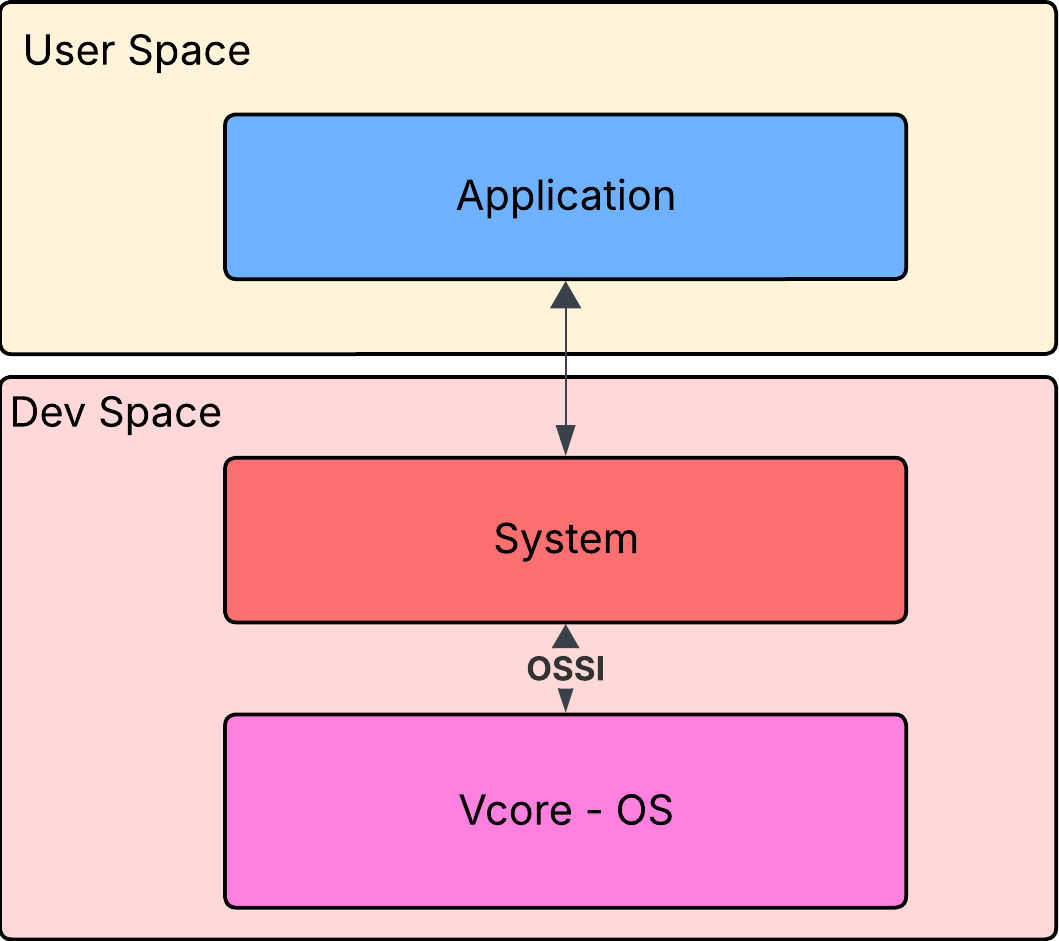
\includegraphics[width=0.45\linewidth]{Textuais/Imgs/Metodologia/Diagrama_sistema_completo.png}
    \label{fig:Metodologia_Diagrama_placas}
    
    \small Fonte: Autor (2026)
\end{figure}

Toda a comunicação interprocessos (IPC) do sistema é padronizada pelo OSSI (\textit{Operating System Standard Interface}). Este módulo atua como um barramento roteador de dados baseado em filas de mensagens (\textit{message queues}). Para garantir um tráfego seguro e determinístico, o OSSI utiliza passagem por valor para comandos internos — evitando alocação dinâmica e fragmentação do \textit{heap} — e passagem por referência para pacotes extensos de rede.

A camada \textit{Vcore - OS} atua como a infraestrutura fundacional do sistema. Sua principal função é encapsular as rotinas nativas do \textit{Zephyr} OS, isolando a lógica de aplicação das complexidades de \textit{hardware} e dos protocolos de rede. A estrutura interna desta camada está detalhada na \autoref{fig:Metodologia_Vcore}.

\begin{figure}[H]
    \centering
    \caption{Diagrama de blocos da camada \textit{Vcore - OS}}
    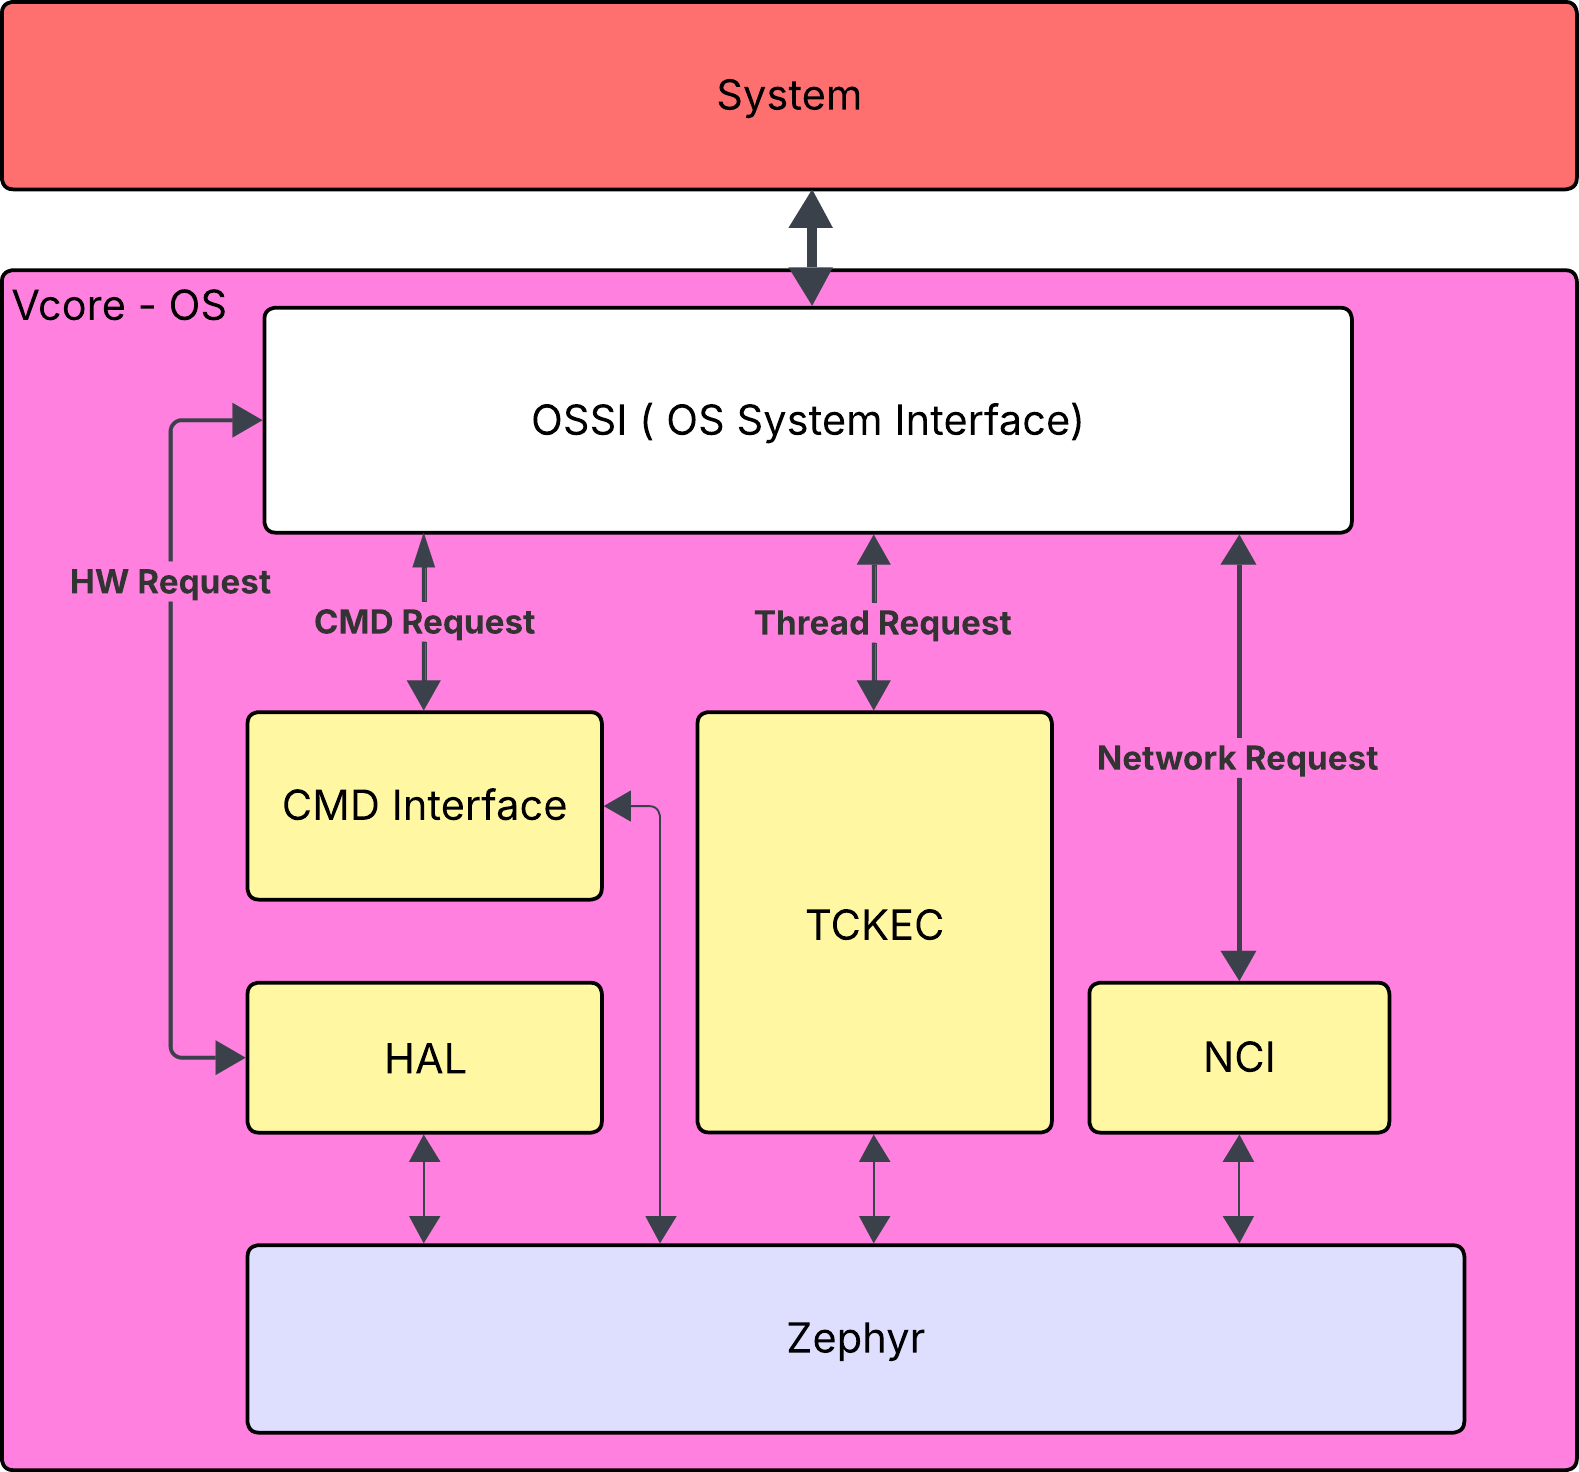
\includegraphics[width=0.45\linewidth]{Textuais/Imgs/Metodologia/Vcore.png}
    \label{fig:Metodologia_Vcore}
    
     Fonte: Autor (2026)
\end{figure}

Os principais módulos que compõem o \textit{Vcore - OS} são:
\begin{itemize}
    \item \textbf{CMD:} Interpretador central que recebe pacotes binários brutos da rede, valida as instruções e roteia os comandos para o subsistema responsável.
    \item \textbf{TCKEC (\textit{Thread Create Kill Executive Control}):} Gerenciador do ciclo de vida dos processos. Centraliza a criação e a destruição dinâmica de \textit{threads}, otimizando o gerenciamento de recursos e de energia da CPU.
    \item \textbf{NCI (\textit{Network Core Interface}):} Gerenciador da pilha de rede UDP e do \textit{socket} de comunicação, responsável por garantir a recepção e a transmissão de dados com latência minimizada.
    \item \textbf{HAL (\textit{Hardware Abstraction Layer}):} Interface de comunicação direta com os periféricos do microcontrolador (como o ADC operando via DMA para leituras analógicas em \textit{background}), isolando os registradores físicos das camadas superiores.
\end{itemize}


\section{Montagem Mecânica e Elétrica da Bancada de Aquisição}

A arquitetura da bancada de aquisição foi organizada em uma estrutura funcional hierárquica, conforme apresentado no diagrama da Figura~\ref{fig:diagrama_blocos}. O sistema integra cinco camadas complementares: alimentação, controle de carga, condicionamento e medição, sensoriamento distribuído e comunicação em rede.

A energia provém de duas fontes intercambiáveis: uma bateria LiPo para operação em ensaios dinâmicos e uma fonte CA/CC de rede elétrica para operação em bancada estacionária. Ambas alimentam um barramento comum de 12V através de diodos em configuração OR lógica, garantindo que a bateria tenha prioridade automática quando conectada, sem necessidade de comutação manual. Deste barramento, dois estágios reguladores buck reduzem a tensão para 12V (alimentação de placas de controle e relés) e 5V (circuitos analógicos e sensores digitais).

O controle da conexão ao motor é realizado por dois relés em sequência: o relé de pré-carga é acionado inicialmente, inserindo um resistor de 100$\,\Omega$ em série com o barramento de alimentação do ESC, limitando a corrente de inrush durante o carregamento dos capacitores internos. Após este período de estabilização, o relé de carga é acionado, efetuando um bypass do resistor de pré-carga e conectando o ESC diretamente ao barramento de potência. Durante esta sequência, um amperímetro registra a corrente total do sistema e um voltímetro monitora continuamente a tensão da bateria.

O ESC comanda o motor BLDC, gerando três fases de corrente ($i_a$, $i_b$, $i_c$). A placa SAME captura os sinais analógicos de corrente, bem como sinais de tensão de linha para posterior reconstrução da componente de tensão neutra via transformação de Clarke. 

Simultaneamente, a placa SIBA controle o PPM para acionamento do ESC, os relés de pré-carga e de carga, além das leituras, do RPM, Bateria e Tubo de pitot, via I2C (\textit{Inter-Integrated Circuit}), como também das células de carga, via \textit{bit banging} e das temperaturas da bateria e motor.

 Um switch Ethernet interno interconecta as placas SAME, SIBA e um computador externo, viabilizando aquisição sincronizada em tempo real via protocolo NCI transportado por UDP, que permite a transmissão de dados de forma isolada e com multiplos nós de operação.

\begin{figure}[htb]
    \centering
    % \includegraphics[width=0.85\textwidth]{figuras/diagrama_blocos}
    \caption{Diagrama de blocos da arquitetura de aquisição}
    \label{fig:diagrama_blocos}

    \begin{tikzpicture}[transform shape, american voltages, scale=0.7]
	% Paths, nodes and wires:
	\node[fourport, xscale=1.55, yscale=1.55](ESC) at (14.04, 9.079){} node[anchor=center] at (ESC.center){$\text{ESC}$};
	\node[fourport](N1) at (17.489, 9.039){} node[anchor=center] at (N1.center){$\text{Aquisição}$};
	\node[shape=circle, draw, line width=1pt, minimum width=1.465cm](N2) at (20.27, 9.07){} node[anchor=center] at (N2.text){$\text{BLDC}$};
	\draw (2.121, 9.949) to[battery, l={$V_{bateria}$}] (2.121, 7.449);
	\node[ground] at (2.121, 7.449){};
	\draw (2.121, 7.699) -| (2.121, 7.449);
	\draw (16.579, 9.494) |- (15.489, 9.539);
	\draw (16.579, 8.584) |- (15.489, 8.539);
	\draw (15.489, 9.039) -| (16.591, 9.017);
	\node[shape=rectangle, minimum width=0.715cm, minimum height=0.215cm](N3) at (16.114, 9.789){} node[anchor=center] at (N3.text){$i_a$};
	\node[shape=rectangle, minimum width=0.715cm, minimum height=0.215cm](N4) at (16.114, 9.289){} node[anchor=center] at (N4.text){$i_b$};
	\node[shape=rectangle, minimum width=0.715cm, minimum height=0.215cm](N5) at (16.114, 8.789){} node[anchor=center] at (N5.text){$i_c$};
	\draw (19.621, 9.449) |- (18.399, 9.494);
	\draw (19.739, 8.539) |- (18.399, 8.494);
	\draw (18.399, 8.994) -| (19.489, 9.039);
	\node[shape=rectangle, minimum width=0.715cm, minimum height=0.215cm](N6) at (19.024, 9.744){} node[anchor=center] at (N6.text){$i_a$};
	\node[shape=rectangle, minimum width=0.805cm, minimum height=0.295cm](N7) at (19.069, 9.204){} node[anchor=center] at (N7.text){$i_b$};
	\node[shape=rectangle, minimum width=0.715cm, minimum height=0.215cm](N8) at (19.024, 8.744){} node[anchor=center] at (N8.text){$i_c$};
	\draw (10.951, 10.374) to[ammeter] (11.951, 10.374);
	\draw (4.121, 8.199) to[voltmeter] (4.121, 9.449);
	\draw (7.607, 9.874) to[cute open switch, mirror, l={$\text{Relé de carga}$}] (6.107, 9.874);
	\draw (7.607, 10.874) to[cute open switch, mirror, l={$\text{Relé de pré-carga}$}] (6.107, 10.874);
	\draw (8.201, 10.874) to[american resistor, l={$100 \Omega$}] (9.951, 10.874);
	\draw (6.107, 9.874) |- (5.451, 9.874) |- (6.107, 10.874);
	\draw (7.607, 10.874) -- (8.201, 10.874);
	\draw (7.607, 9.874) -- (9.951, 9.874) -| (9.951, 10.874);
	\draw (9.951, 10.374) -- (10.951, 10.374);
	\draw (11.951, 10.374) -| (12.201, 9.874) -| (12.63, 9.784);
	\draw (2.121, 9.949) -| (2.121, 10.449) -- (4.121, 10.449);
	\draw (4.121, 9.949) -| (4.121, 9.449);
	\draw (4.121, 8.199) |- (2.121, 7.449);
	\draw (4.121, 9.949) -| (4.121, 10.449);
	\draw (4.121, 10.449) -- (5.371, 10.449);
	\draw (4.121, 7.449) -| (12.121, 8.199) |- (12.63, 8.374);
	\draw (1.941, 6.039) to[sinusoidal voltage source] (1.941, 3.539);
	\node[fourport](N9) at (4.781, 4.994){} node[anchor=center] at (N9.center){$AC/DC$};
	\draw (1.941, 3.539) -- (2.941, 3.539) -| (3.191, 4.539) -| (3.871, 4.539);
	\draw (3.871, 5.449) |- (3.191, 5.539) -- (3.191, 6.039) -- (1.941, 6.039);
	\draw (6.441, 5.449) to[empty diode] (8.191, 5.449);
	\node[ground] at (6.441, 4.199){};
	\draw (6.441, 4.199) -| (6.441, 4.449) |- (5.691, 4.539);
	\draw (5.691, 5.449) -- (6.441, 5.449);
	\node[fourport](N10) at (17.461, 4.404){} node[anchor=center] at (N10.center){$\text{SIBA}$};
	\node[fourport, xscale=1.03, yscale=1.03](N11) at (17.383, 6.731){} node[anchor=center] at (N11.center){$\text{SAME}$};
	\draw (4.986, 6.645) to[empty diode] (6.736, 6.645);
	\draw (6.736, 6.645) to[sdcdc] (8.986, 6.645);
	\draw (9.736, 6.645) -- (8.986, 6.645);
	\node[shape=rectangle, minimum width=0.965cm, minimum height=0.465cm] at (9.121, 6.949){} node[anchor=north west, align=left, text width=0.577cm, inner sep=6pt] at (8.621, 7.199){$12V$};
	\draw (10.756, 6.645) to[sdcdc] (13.006, 6.645);
	\node[shape=rectangle, minimum width=0.715cm, minimum height=0.465cm] at (15.025, 6.9){} node[anchor=north west, align=left, text width=0.327cm, inner sep=6pt] at (14.65, 7.15){$5V$};
	\draw (13.006, 6.645) to[empty diode] (14.756, 6.645);
	\draw (9.736, 6.645) to[normal open switch, l={$\text{Chave}$}] (10.736, 6.645);
	\draw (4.986, 6.645) -- (4.621, 6.645) -- (4.621, 10.449);
	\draw (8.191, 5.449) -| (14.756, 6.645);
	\draw (16.921, 8.099) -| (16.921, 7.699);
	\draw (17.421, 7.699) -| (17.421, 8.099);
	\draw (17.921, 8.099) -| (17.921, 7.699);
	\draw (16.521, 4.399) -| (15.5, 6.6);
	\node[circ] at (4.121, 10.449){};
	\node[circ] at (4.621, 10.449){};
	\node[circ] at (9.951, 10.374){};
	\node[circ] at (14.756, 6.645){};
	\node[circ] at (15.521, 6.599){};
	\node[circ] at (16.921, 8.099){};
	\node[circ] at (16.921, 7.699){};
	\node[circ] at (17.421, 7.699){};
	\node[circ] at (17.421, 8.099){};
	\node[circ] at (17.921, 8.099){};
	\node[circ] at (17.921, 7.699){};
	\node[jump crossing] at (15.9, 6.64){};
	\draw (16.04, 6.64) -| (16.4, 6.7);
	\draw (15.456, 6.645) -- (14.756, 6.645);
	\draw (15.456, 6.645) -| (15.76, 6.64);
	\draw (15.9, 6.5) -| (15.9, 5.2) -- (15.9, 4.9) |- (16.551, 4.859);
	\draw (15.9, 6.78) |- (15.5, 7.9);
	\node[shape=rectangle, minimum width=0.965cm, minimum height=0.365cm] at (15.9, 8.2){} node[anchor=north west, align=left, text width=0.577cm, inner sep=6pt] at (15.4, 8.4){PPM};
	\node[fourport, xscale=1.49, yscale=1.49](N12) at (20.844, 5.278){} node[anchor=center] at (N12.center){$\textit{Switch} \ \text{de Rede}$};
	\draw (18.4, 4.7) -- (19.1, 4.7) -| (19.488, 4.644);
	\draw (18.321, 6.262) -| (18.9, 6) -- (19.488, 6);
	\node[fourport, xscale=1.09, yscale=1.09](N13) at (20.892, 2.004){} node[anchor=center] at (N13.center){$\text{PC Externo}$};
	\draw (20.9, 3) -| (20.9, 3.9);
	\node[shape=rectangle, minimum width=0.665cm, minimum height=0.365cm] at (18.75, 5.1){} node[anchor=north west, align=left, text width=0.277cm, inner sep=6pt] at (18.4, 5.3){ETH};
	\node[shape=rectangle, minimum width=0.665cm, minimum height=0.365cm] at (18.7, 6.8){} node[anchor=north west, align=left, text width=0.277cm, inner sep=6pt] at (18.35, 7){ETH};
	\node[shape=rectangle, minimum width=0.665cm, minimum height=0.365cm] at (20.15, 3.4){} node[anchor=north west, align=left, text width=0.277cm, inner sep=6pt] at (19.8, 3.6){ETH};
	\node[shape=rectangle, draw, line width=1pt, minimum width=1.265cm, minimum height=1.165cm] at (11.95, 4.2){} node[anchor=center, align=center, text width=0.877cm, inner sep=6pt] at (11.95, 4.2){\small Bateria};
	\node[shape=rectangle, draw, line width=1pt, minimum width=1.365cm, minimum height=1.64cm] at (18, 1.337){} node[anchor=center, align=center, text width=0.977cm, inner sep=6pt] at (18, 1.337){\scriptsize Células de Carga};
	\node[shape=rectangle, draw, line width=1pt, minimum width=1.365cm, minimum height=1.165cm] at (10.3, 4.2){} node[anchor=center, align=center, text width=0.977cm, inner sep=6pt] at (10.3, 4.2){RPM};
	\node[shape=rectangle, draw, line width=1pt, minimum width=2.265cm, minimum height=1.165cm] at (14.05, 4.2){} node[anchor=center, align=center, text width=1.997cm, inner sep=4.3pt] at (14.05, 4.2){\footnotesize Tubo de Pitot};
	\draw (16.5, 4.2) -- (15.5, 4.2) |- (10.3, 3.1);
	\draw (10.3, 3.6) -| (10.3, 3.1);
	\draw (11.95, 3.6) |- (12, 3.1);
	\draw (13.6, 3.6) -- (13.6, 3.1);
	\node[shape=rectangle, minimum width=0.865cm, minimum height=0.565cm] at (11.95, 2.8){} node[anchor=north west, align=left, text width=0.477cm, inner sep=6pt] at (11.5, 3.1){I2C};
	\draw (18, 3.5) -- (18, 2.2);
	\node[shape=rectangle, draw, line width=1pt, minimum width=1.265cm, minimum height=1.165cm] at (10.4, 1.8){} node[anchor=center, align=center, text width=0.877cm, inner sep=6pt] at (10.4, 1.8){\small Relés\\};
	\node[shape=rectangle, draw, line width=1pt, minimum width=2.065cm, minimum height=1.165cm] at (12.7, 1.8){} node[anchor=center, align=center, text width=1.677cm, inner sep=6pt] at (12.7, 1.8){\scriptsize Temperaturas};
	\draw (16.551, 3.949) |- (15.8, 3.9) |- (13.8, 1.8) -- (13.75, 1.8);
	\draw (16.9, 3.5) |- (15, 1.5) |- (14.9, 1) -| (10.4, 1.2);
\end{tikzpicture}

    Fonte: Autor(2026)

\end{figure}

\subsection{Dimensionamento do Resistor de Pré-carga}

O valor do resistor de pré-carga foi determinado a partir da constante de tempo
$RC$ do circuito formado pelo próprio resistor e pela capacitância equivalente
de entrada do ESC. Adotou-se como critério que o carregamento dos capacitores
atinja o regime permanente, definido como cinco constantes de tempo
($99{,}3\%$ da tensão de barramento), em um intervalo de \SI{1}{\second},
garantindo a limitação da corrente de inrush sobre os contatos do relé de
pré-carga sem comprometer a sequência de acionamento.

A constante de tempo do circuito é dada por

\begin{equation}
    \tau = R_{pc} \, C_{ESC},
    \label{eq:tau_precarga}
\end{equation}

\noindent onde $R_{pc}$ é a resistência de pré-carga e $C_{ESC}$ a capacitância
equivalente de entrada do ESC. Impondo o critério de tempo total de pré-carga
$t_{pc} = 5\tau = \SI{1}{\second}$, obtém-se a constante de tempo requerida

\begin{equation}
    \tau = \frac{t_{pc}}{5} = \frac{\SI{1}{\second}}{5} = \SI{0,2}{\second}.
    \label{eq:tau_valor}
\end{equation}

Considerando $C_{ESC} = \SI{2000}{\micro\farad}$, a resistência de pré-carga resulta em

\begin{equation}
    R_{pc} = \frac{\tau}{C_{ESC}} = \frac{\SI{0,2}{\second}}{\SI{2000}{\micro\farad}} = \SI{100}{\ohm}.
    \label{eq:rpc_valor}
\end{equation}

A corrente de pico durante a pré-carga ocorre no instante inicial ($t = 0$),
quando a tensão sobre os capacitores é nula e toda a tensão de barramento se
aplica ao resistor. Para a bateria LiPo de 6 células plenamente carregada
($V_{max} = \SI{25,2}{\volt}$), tem-se

\begin{equation}
    I_{pico} = \frac{V_{max}}{R_{pc}} = \frac{\SI{25,2}{\volt}}{\SI{100}{\ohm}} = \SI{252}{\milli\ampere}.
    \label{eq:ipico}
\end{equation}

Esta corrente é significativamente inferior à capacidade de comutação do relé de
pré-carga, dispensando qualquer preocupação com desgaste ou solda dos contatos.

A potência dissipada pelo resistor é máxima também em $t = 0$ e decai
exponencialmente ao longo do carregamento, à medida que a tensão sobre o
resistor diminui. A dissipação instantânea de pico é

\begin{equation}
    P_{pico} = \frac{V_{max}^2}{R_{pc}} = \frac{\left(\SI{25,2}{\volt}\right)^2}{\SI{100}{\ohm}} \approx \SI{6,35}{\watt}.
    \label{eq:ppico}
\end{equation}


\subsection{Caixa de Instrumentação}

A integração dos sistemas SAME e SIBA foi realizada em uma caixa de
instrumentação fabricada por impressão 3D em filamento PLA, projetada para
centralizar a alimentação, o processamento e as conexões de sinal em um único
módulo físico. A escolha da impressão 3D permitiu a prototipagem rápida de uma
geometria customizada às necessidades do projeto, com fixação interna dedicada
para cada subsistema. Por se tratar de ensaios de curta duração, a limitação
térmica do PLA não compromete a operação; ainda assim, previram-se aberturas
para dissipação do calor gerado pelos componentes de potência.

\subsection{Organização Interna}

O \textit{layout} interno foi organizado de forma a separar fisicamente os
componentes de potência dos circuitos de medição, minimizando o acoplamento
eletromagnético entre eles. Tal separação é particularmente crítica neste
projeto, uma vez que os sinais de interesse são de baixa amplitude — como a
queda de tensão da ordem de milivolts sobre resistências de poucos
miliohms e a saída dos sensores de efeito Hall —, sendo, portanto,
suscetíveis a interferência. As placas SAME e SIBA foram fixadas nas
extremidades da caixa por meio de parafusos, enquanto a placa de
condicionamento de sinal do motor foi posicionada na região central,
equidistante das duas placas principais. O ESC foi fixado internamente por
abraçadeiras de náilon, garantindo imobilidade mecânica durante os ensaios
sem danificar o encapsulamento do componente.

O \textit{switch} Ethernet foi instalado internamente, com as portas RJ45
acessíveis pelo painel externo da caixa, permitindo a conexão com a rede de
aquisição sem necessidade de abertura do gabinete.

\subsection{Conexões Externas}

O painel externo da caixa concentra todas as interfaces com o ambiente de
ensaio. O conector XT90 de entrada recebe a bateria LiPo, enquanto um segundo
conector XT90 de saída alimenta o ESC. Os fios de fase do motor passam pelo
interior da caixa através de conectores \textit{bullet} de \SI{6}{\milli\meter},
permitindo a interposição dos núcleos de ferrite para a medição de corrente sem
interrupção do cabo de potência. Uma entrada dedicada no painel permite a
conexão dos fios da célula de carga utilizada para a medição de força de tração
na bancada aerodinâmica.

\section{SIBA - Sistema Integrado da Bancada Aerodinâmica}
O SIBA atua como o nó central de aquisição da bancada, sendo responsável pela interface com os sensores aerodinâmicos, gestão da energia e coordenação da rede de dados. Sua metodologia de desenvolvimento foi dividida em infraestrutura de \textit{hardware} e lógica de controle embarcada.


\subsection{\textit{Hardware}}


\subsection{\textit{Firmware}}

\subsubsection{Camada \textit{System}}

O \textit{System} representa a camada de lógica de negócios do sistema, o \textit{Thread} \textit{System Manager} é o responsável por processar os dados dos sensores e executar os comandos de controle. A Figura \ref{fig:Metodologia_SystemManager_Siba} detalha a composição deste gerenciador.

\begin{figure}[H]
    \centering
    \caption{Diagrama de blocos do \textit{System}}
    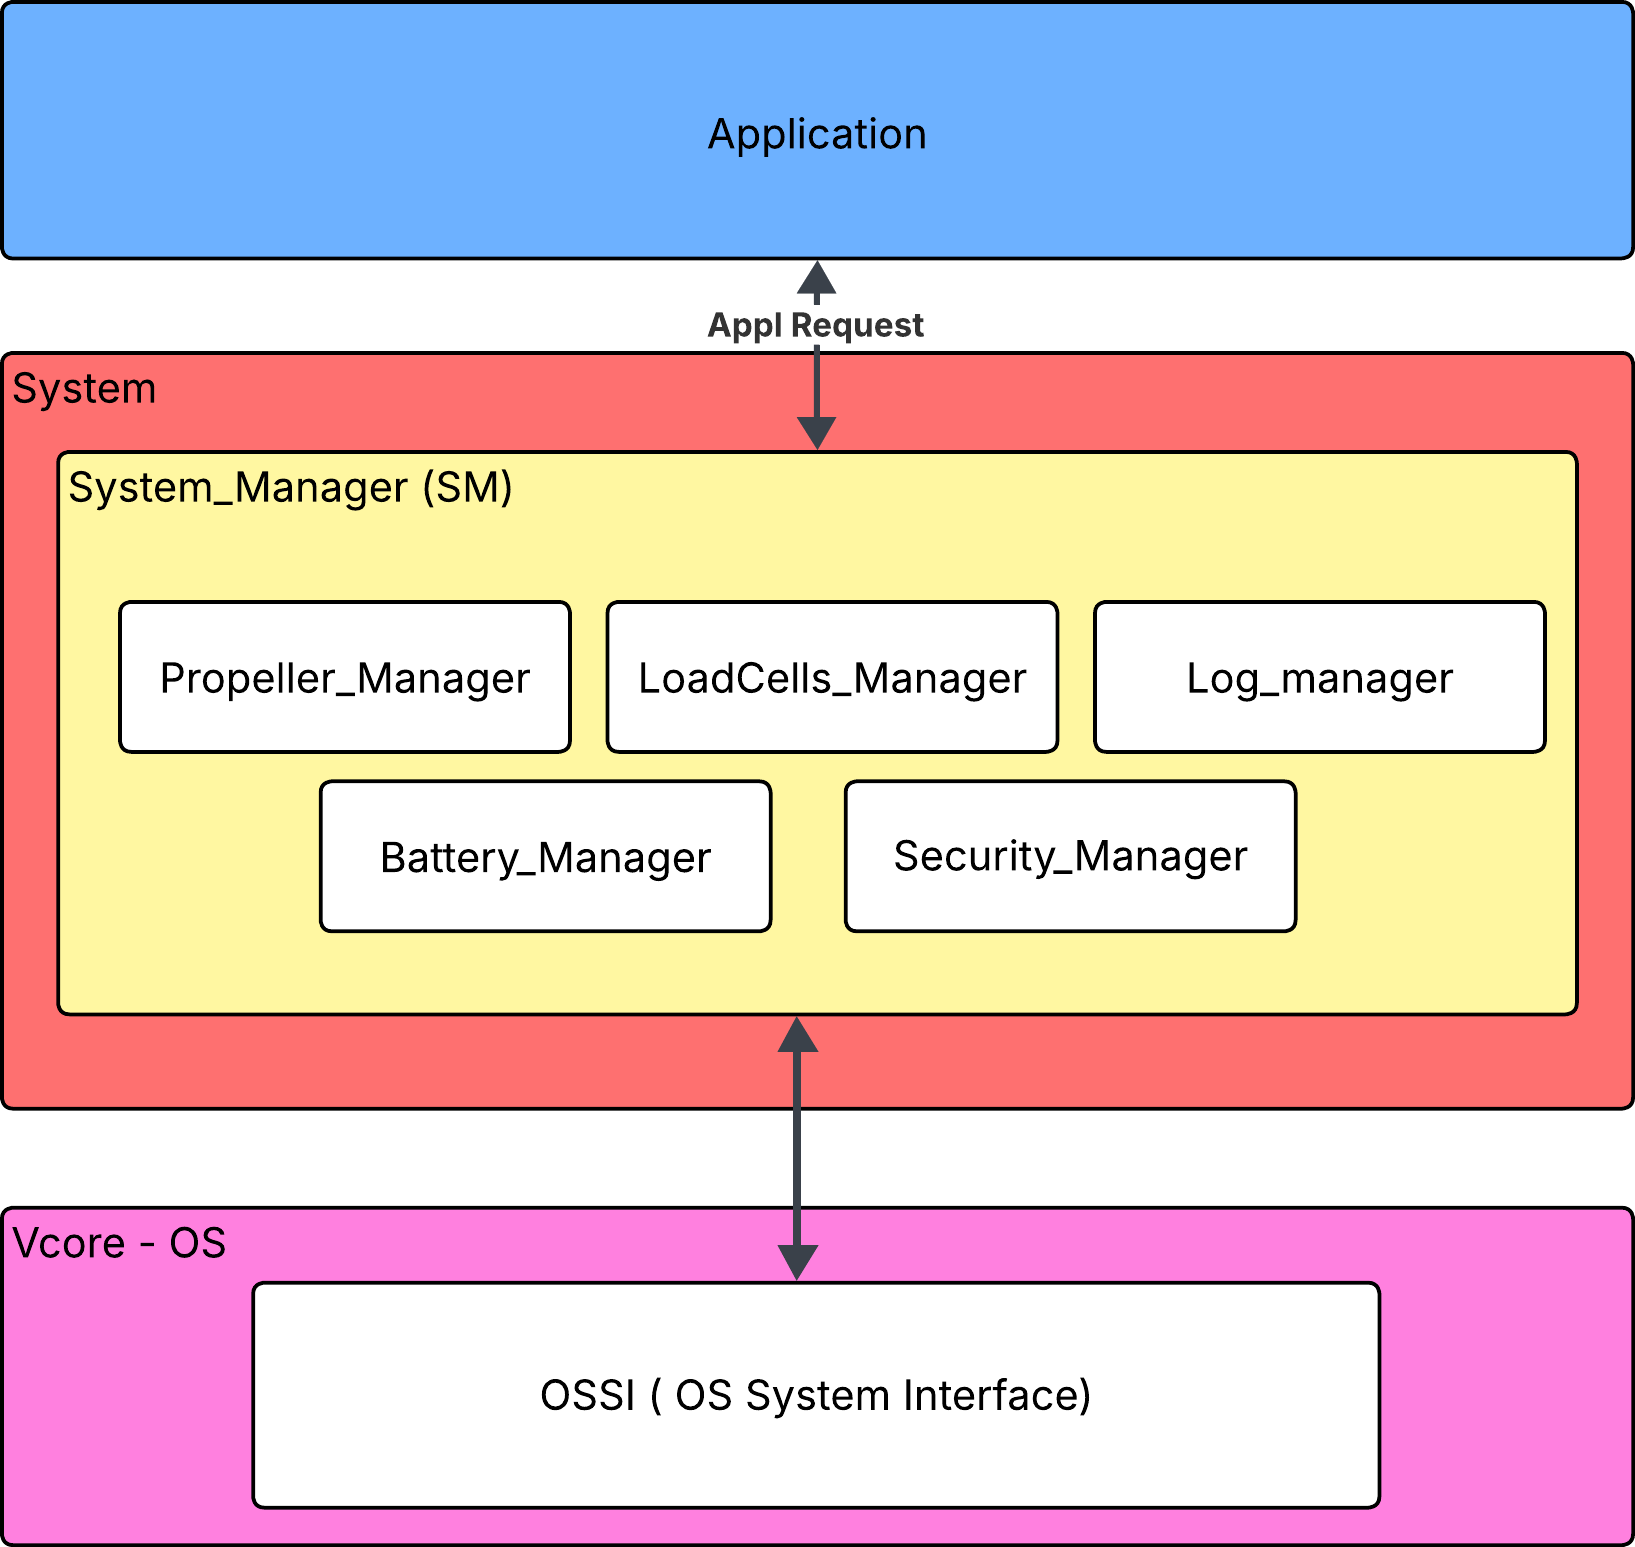
\includegraphics[width=0.6\linewidth]{Textuais/Imgs/Metodologia/SystemManager.png}
    \label{fig:Metodologia_SystemManager_Siba}
    
    Fonte: Autor (2026)
\end{figure}

Esta camada opera no espaço de desenvolvimento e gerencia os seguintes subsistemas internos ao Thread:
\begin{itemize}
    \item \textbf{\textit{Propeller Manager}:} Gerencia os parâmetros da hélice, como a medição de RPM (utilizando o modo \textit{Input Capture} dos temporizadores em \textit{hardware} puro) e o cálculo de tração via célula de carga.
    \item \textbf{\textit{Battery Manager}:} Realiza o monitoramento da interface de alimentação, processando dados de tensão e corrente para estimativa de potência de entrada.
    \item \textbf{\textit{Security Manager}:} Monitora continuamente os limites de operação (como sobrecorrente ou temperaturas críticas), garantindo o desligamento ou limitação de potência em situações de risco.
    \item \textbf{\textit{Log Manager}:} Responsável pela telemetria do sistema. Emprega a técnica de agregação de dados (\textit{batching}) para empacotar respostas de comandos e leituras de sensores em um único vetor, otimizando o uso da banda de rede ao enviar os dados de volta para a estação de controle.
\end{itemize}

Por fim, a camada de \textbf{\textit{Application}} opera isolada no \textit{User Space} (espaço de usuário). No ambiente do RTOS \textit{Zephyr} executado na arquitetura RISC-V, este isolamento é garantido por \textit{hardware} através da unidade de Proteção de Memória Física (PMP - \textit{Physical Memory Protection}). Essa restrição de níveis de privilégio assegura que a Aplicação não possua acesso direto aos registradores físicos ou aos endereços de memória restritos das camadas \textit{System} e \textit{Vcore - OS}. Qualquer interação ou requisição para as camadas inferiores ocorre estritamente de forma segura e controlada através do barramento central de comunicação (OSSI), o que garante que eventuais falhas na camada de aplicação não comprometam a estabilidade do núcleo do sistema.



\section{SAME - Sistema de Aquisição do Motor Elétrico}
\label{sec:same}

O desenvolvimento do Sistema de Aquisição do Motor Elétrico (SAME) teve como
foco o projeto de um hardware dedicado para medição elétrica e a execução
embarcada do Observador por Modos Deslizantes (SMO). A seleção de componentes e
o roteamento da placa de circuito impresso (PCB) foram orientados por três
critérios metodológicos fundamentais:

\begin{enumerate}
    \item \textbf{Custo global da solução:} priorizou-se a seleção de
    componentes com alto grau de integração, reduzindo a necessidade de
    circuitos de condicionamento externos e minimizando o número de camadas da
    PCB, o que viabilizou a prototipagem iterativa.

    \item \textbf{Espaço ocupado (\textit{Footprint}):} as restrições de área na
    bancada exigiram a adoção de componentes de montagem em superfície (SMD) e
    roteamento de alta densidade. O módulo precisava ser compacto o suficiente
    para ser posicionado próximo às fases do motor sem interferir no escoamento
    de ar gerado pela hélice.

    \item \textbf{Disponibilidade de mercado:} a consolidação da lista de
    materiais (BOM --- \textit{Bill of Materials}) foi atrelada aos estoques
    ativos de fornecedores e linhas de montagem (PCBA), mitigando o risco de
    atrasos por escassez de silício ou componentes passivos críticos.
\end{enumerate}

A cadeia de medição foi dividida em dois caminhos independentes --- corrente e
tensão de fase ---, cada um projetado para entregar ao conversor
analógico-digital (ADC) do CH32V307 um sinal na faixa de entrada do periférico,
preservando a coerência de fase entre os dois caminhos exigida pelo observador
(\autoref{sec:condicionamento}).


\subsection{Medição de Tensão e Corrente de Fase}
\label{sec:same_tensao}

O sistema de aquisição utiliza dois conversores ADC operando em paralelo no CH32V307 com frequência de clock ADC de 14~MHz, conforme Tabela~4-40 do datasheet \cite{ch32v307_datasheet}. Cada módulo opera a taxa máxima de 1~MSps, com ADC1 digitalizando as três tensões de fase e ADC2 capturando as três correntes de fase de forma entrelançada, alcançando aproximadamente 333~kSps por canal. Esta taxa é escolhida para amostrar bem acima da frequência de chaveamento do ESC (16~kHz) e capturar a dinâmica do motor em operação, garantindo que o teorema de amostragem de Nyquist seja satisfeito \cite{oppenheim2009}.

\begin{table}[h]
\centering
\caption{Características do ADC 12-bit do CH32V307.}
\label{tab:adc_specs}
\begin{tabular}{lccccc}
\hline
\textbf{Parâmetro} & \textbf{Símbolo} & \textbf{Min.} & \textbf{Typ.} & \textbf{Máx.} & \textbf{Unidade} \\
\hline
Frequência de clock ADC & $f_{ADC}$ & -- & -- & 14 & MHz \\
Taxa de amostragem & $f_S$ & 0,05 & -- & 1 & MHz \\
Tensão de referência & $V_{REF+}$ & 2,4 & -- & $V_{DDA}$ & V \\
Faixa de conversão & $V_{AIN}$ & 0 & -- & $V_{REF+}$ & V \\
Corrente de referência & $I_{VREF}$ & 160 & 220 & -- & $\mu$A \\
Corrente de alimentação & $I_{DDA}$ & 480 & 530 & -- & $\mu$A \\
Impedância de entrada externa & $R_{AIN}$ & -- & -- & 50 & k$\Omega$ \\
Tempo de calibração & $t_{CAL}$ & -- & 40 & -- & $1/f_{ADC}$ \\
Tempo de amostragem & $t_s$ & 1,5 & -- & 239,5 & $1/f_{ADC}$ \\
Tempo total de conversão & $t_{CONV}$ & 14 & -- & 252 & $1/f_{ADC}$ \\
\hline
\multicolumn{6}{l}{\small \textit{Fonte: WCH CH32V307 Datasheet \cite{ch32v307_datasheet}}} \\
\end{tabular}
\end{table}

Com clock de 14~MHz, o tempo total de conversão varia entre 1~$\mu$s (14 ciclos) e 18~$\mu$s (252 ciclos). Como o período de PWM em 16~kHz é de 62,5~$\mu$s e cada ADC realiza apenas 3 conversões por período, há folga suficiente para adotar tempo de amostragem $t_s$ elevado, priorizando o assentamento do sinal em detrimento da velocidade bruta.

A impedância de entrada externa $R_{AIN}$ deve ser limitada para garantir que o erro de amostragem permaneça abaixo de 1/4 LSB, conforme a \autoref{eq:rain_max} \cite{ch32v307_datasheet}.

\begin{equation}
R_{AIN} < \frac{t_s}{f_{ADC} \cdot C_{ADC} \cdot \ln(2^{N+2})} - R_{ADC}
\label{eq:rain_max}
\end{equation}

onde $N = 12$~bits, $C_{ADC} = 8$~pF e $R_{ADC} \approx 0{,}8$~k$\Omega$. Esta relação é determinante para o projeto do divisor de tensão: a impedância equivalente de Thévenin vista pela entrada do ADC ($R_1 \parallel R_2$) deve respeitar os limites da Tabela~\ref{tab:rain_max}. Adotando $t_s = 55{,}5$~ciclos (3,96~$\mu$s), $R_{AIN}$ pode chegar a 50~k$\Omega$, relaxando a escolha dos resistores; já com $t_s = 13{,}5$~ciclos, o divisor precisa apresentar impedância abaixo de 11,4~k$\Omega$ sob pena de erro de conversão.

\begin{table}[h]
\centering
\caption{Impedância máxima de entrada externa em função do tempo de amostragem.}
\label{tab:rain_max}
\begin{tabular}{ccc}
\hline
\textbf{$t_s$ (ciclos)} & \textbf{$t_s$ ($\mu$s)} & \textbf{$R_{AIN}^{\text{máx}}$ (k$\Omega$)} \\
\hline
1,5 & 0,11 & 0,4 \\
7,5 & 0,54 & 5,9 \\
13,5 & 0,96 & 11,4 \\
28,5 & 2,04 & 25,2 \\
41,5 & 2,96 & 37,2 \\
55,5 & 3,96 & 50,0 \\
\hline
\multicolumn{3}{l}{\small \textit{Fonte: WCH CH32V307 Datasheet \cite{ch32v307_datasheet}}} \\
\end{tabular}
\end{table}

Os erros inerentes ao ADC de 12 bits são especificados na Tabela~\ref{tab:adc_error}. O offset de ±2~LSB é tipicamente removível via calibração, enquanto as não-linearidades diferenciais e integrais representam limitações do circuito integrado. Para $R_{AIN} < 10$~k$\Omega$, o erro total esperado é de aproximadamente ±4~LSB em condição de pior caso.

\begin{table}[h]
\centering
\caption{Erros de conversão do ADC 12-bit em operação típica.}
\label{tab:adc_error}
\begin{tabular}{lccc}
\hline
\textbf{Parâmetro} & \textbf{Símbolo} & \textbf{Typ.} & \textbf{Máx.} \\
\hline
Erro de offset & $E_O$ & 0 & ±2 LSB \\
Não-linearidade diferencial & $E_D$ & -- & ±3 LSB \\
Não-linearidade integral & $E_L$ & -- & ±4 LSB \\
\hline
\multicolumn{4}{l}{\small \textit{Fonte: WCH CH32V307 Datasheet \cite{ch32v307_datasheet}}} \\
\end{tabular}
\end{table}

\subsubsection{Condicionamento de Sinal}

A tensão de barramento (até 25~V em bateria 6S) é reduzida através de um divisor resistivo para cair na faixa de entrada do ADC (0--3,3 V), conforme a Equação~\eqref{eq:divisor_tensao} \cite{analog_signal_conditioning}:

\begin{equation}
V_{ADC} = V_{fase} \cdot \frac{R_2}{R_1 + R_2}
\label{eq:divisor_tensao}
\end{equation}

Um filtro RC antialiasing de primeira ordem é posicionado na saída do divisor com frequência de corte:

\begin{equation}
f_c = \frac{1}{2\pi RC}
\label{eq:fc_antialiasing}
\end{equation}

escolhida em torno de 40--50~kHz. O objetivo é atenuar componentes de frequência acima da frequência de Nyquist ($f_{\text{Ny}} = f_s / 2 \approx 56~\text{kHz}$) que não contêm informação útil sobre o motor mas carregam ruído de chaveamento (16~kHz e seus harmônicos). A atenuação de ~40 dB/década do filtro de primeira ordem elimina efetivamente o ruído PWM mantendo a banda passante dinâmica do motor intacta, um compromisso clássico em acionamentos de potência \cite{franco_opamps}.

A corrente de fase é medida por sensor Hall, que fornece uma tensão proporcional à corrente \cite{allegro_hall_sensors}:

\begin{equation}
V_{out} = V_{ref} + S_H \cdot I_{fase}
\label{eq:hall_corrente}
\end{equation}

onde $V_{ref}$ é o nível de repouso e $S_H$ é a sensibilidade em mV/A. A saída do sensor é acoplada diferencialmente ao ADC2 para rejeição de ruído de modo comum dos cabos de potência, uma prática padrão em acionamentos trifásicos \cite{bldc_control}.

Na Figura~\ref{fig:sampling_adc}, os pontos vermelhos representam as amostras discretas capturadas pelo ADC, cujo código de saída varia entre 0 e $2^{12}-1 = 4095$. As linhas verticais (\textit{stems}) evidenciam a natureza discreta da amostragem: a cada instante de conversão, o sinal analógico contínuo (linha azul) é quantizado em um valor digital inteiro. 

\begin{figure}[h]
\centering
\caption{Ilustração da amostragem dos ADCs.}
\label{fig:sampling_adc}
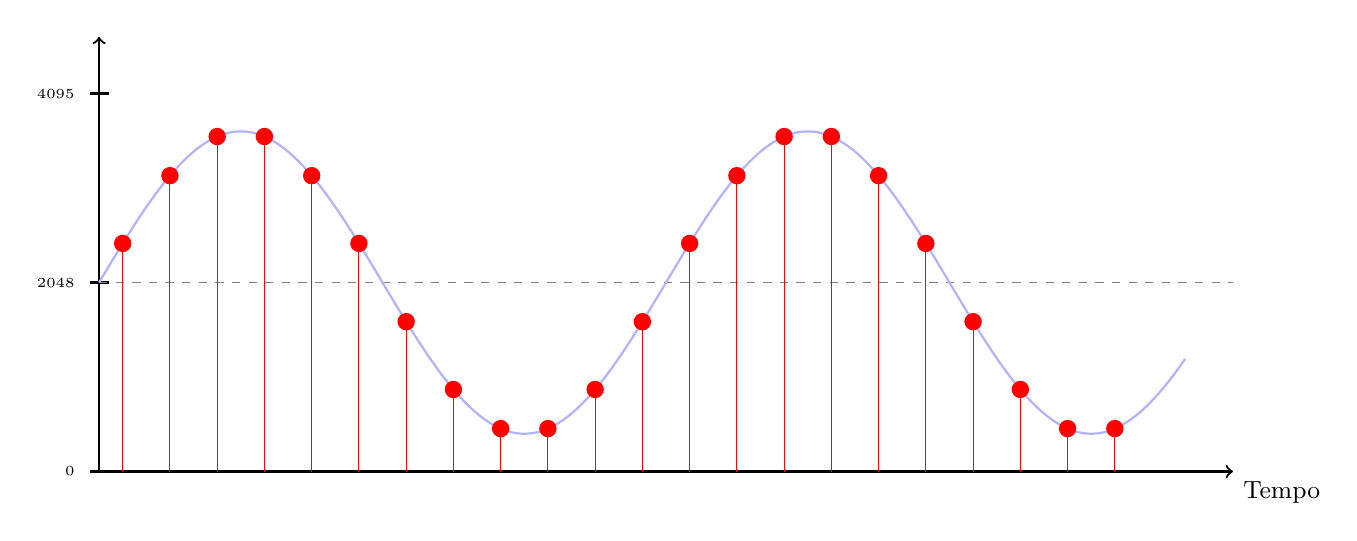
\begin{tikzpicture}[scale=1.2, thick]

  % Parametros: sinal centrado em 2048, amplitude 1600, faixa 0..4095
  % Eixo Y normalizado: 0 -> 0 ; 4095 -> 4 (escala grafica)
  % valor_grafico = (codigo/4095)*4

  % Eixos
  \draw[->] (0, 0) -- (12, 0) node[below right, font=\small] {Tempo};
  \draw[->] (0, 0) -- (0, 4.6) node[left, font=\small] {};

  % Marcas do eixo Y (0, 2048, 4095)
  \foreach \yval/\label in {0/0, 2/2048, 4/4095} {
    \draw (-0.1, \yval) -- (0.1, \yval);
    \node[left, font=\tiny] at (-0.15, \yval) {\label};
  }

  % Linha tracejada no meio de escala (2048)
  \draw[gray, dashed, thin] (0, 2) -- (12, 2);

  % Sinal contínuo original (referência, cinza claro)
  \draw[blue!30, thick, smooth, samples=400, domain=0:11.5]
    plot (\x, {2 + 1.6*sin((\x) * 60)});

  % Stems (linhas verticais até cada amostra) + pontos vermelhos
  \foreach \t in {0.25, 0.75, 1.25, 1.75, 2.25, 2.75, 3.25, 3.75, 4.25, 4.75, 5.25, 5.75, 6.25, 6.75, 7.25, 7.75, 8.25, 8.75, 9.25, 9.75, 10.25, 10.75} {
    \draw[red, thin] (\t, 0) -- (\t, {2 + 1.6*sin((\t) * 60)});
    \filldraw[red, mark size=1.5pt] (\t, {2 + 1.6*sin((\t) * 60)}) circle (0.08);
  }

\end{tikzpicture}

{\small \textit{Fonte: Autor (2026)}}
\end{figure}




\begin{equation}
\text{LSB} = \frac{3.3~\text{V}}{2^{12}} \approx 0.805~\text{mV}
\label{eq:lsb}
\end{equation}

A resolução em unidades físicas (tensão ou corrente) é determinada pela relação de divisão do resistor e pela sensibilidade do sensor Hall, respectivamente. Entretanto, a resolução nominal de 0,805~mV é degradada pelos erros da Tabela~\ref{tab:adc_error}: com não-linearidade integral de até ±4~LSB, a incerteza efetiva de conversão sobe para $\approx 4 \times 0{,}805 = 3{,}2$~mV em pior caso. O erro de offset (±2~LSB) é compensado por calibração via rotina interna do CH32V307 (tempo $t_{CAL} = 40$~ciclos).


